% Format teze zasnovan je na paketu memoir
% http://tug.ctan.org/macros/latex/contrib/memoir/memman.pdf ili
% http://texdoc.net/texmf-dist/doc/latex/memoir/memman.pdf
% 
% Prilikom zadavanja klase memoir, navedenim opcijama se podešava 
% veličina slova (12pt) i jednostrano štampanje (oneside).
% Ove parametre možete menjati samo ako pravite nezvanične verzije
% mastera za privatnu upotrebu (na primer, u b5 varijanti ima smisla 
% smanjiti 
\documentclass[11pt,oneside]{memoir}

% Paket koji definiše sve specifičnosti mastera Matematičkog fakulteta
\usepackage{matfmaster}
\usepackage{amsmath}
\usepackage{float}
\usepackage{xcolor}
\usepackage[normalem]{ulem}
\usepackage{pythonhighlight}

\DeclareMathOperator*{\argmax}{arg\,max}
\DeclareMathOperator*{\argmin}{arg\,min}
%
% Podrazumevano pismo je ćirilica.
%   Ako koristite pdflatex, a ne xetex, sav latinički tekst na srpskom jeziku
%   treba biti okružen sa \lat{...} ili \begin{latinica}...\end{latinica}.
%
% Opicija [latinica]:
%   ako želite da pišete latiniciom, dodajte opciju "latinica" tj.
%   prethodni paket uključite pomoću: \usepackage[latinica]{matfmaster}.
%   Ako koristite pdflatex, a ne xetex, sav ćirilički tekst treba biti
%   okružen sa \cir{...} ili \begin{cirilica}...\end{cirilica}.
%
% Opcija [biblatex]:
%   ako želite da koristite reference na više jezika i umesto paketa
%   bibtex da koristite BibLaTeX/Biber, dodajte opciju "biblatex" tj.
%   prethodni paket uključite pomoću: \usepackage[biblatex]{matfmaster}
%
% Opcija [b5paper]:
%   ako želite da napravite verziju teze u manjem (b5) formatu, navedite
%   opciju "b5paper", tj. prethodni paket uključite pomoću: 
%   \usepackage[b5paper]{matfmaster}. Tada ima smisla razmisliti o promeni
%   veličine slova (izmenom opcije 12pt na 11pt u \documentclass{memoir}).
%
% Naravno, opcije je moguće kombinovati.
% Npr. \usepackage[b5paper,biblatex]{matfmaster}

% Pomoćni paket koji generiše nasumičan tekst u kojem se javljaju sva slova
% azbuke (nema potrebe koristiti ovo u pravim disertacijama)
\usepackage{pangrami}

% Paket koji obezbeđuje ispravni prikaz ćiriličkih italik slova kada
% se koristi pdflatex. Zakomentarisati ako na sistemu koji koristite ovaj
% paket nije dostupan ili ako ne radi ispravno.
\usepackage{cmsrb}

% Ostali paketi koji se koriste u dokumentu
\usepackage{listings} % listing programskog koda
\usepackage{hyperref}

% Ime kandidata na srpskom jeziku (u odabranom pismu)
\autor{Момир Аџемовић}
% Naslov teze na srpskom jeziku (u odabranom pismu)
\naslov{Предвиђање траjекториjа више обjеката на сцени}
% Godina u kojoj je teza predana komisiji
\godina{2022}
% Ime i afilijacija mentora (u odabranom pismu)
\mentor{др Младен Николић, ванредни професор\\ Универзитет у Београду, Математички факултет}
% Ime i afilijacija prvog člana komisije (u odabranom pismu)
\komisijaA{др Јована Ковачевић, доцент\\ Универзитет у Београду, Математички факултет}
% Ime i afilijacija drugog člana komisije (u odabranom pismu)
\komisijaB{др Александар Картељ, доцент\\ Универзитет у Београду, Математички факултет}
% Ime i afilijacija trećeg člana komisije (opciono)
% \komisijaC{}
% Ime i afilijacija četvrtog člana komisije (opciono)
% \komisijaD{}
% Datum odbrane (obrisati ili iskomentarisati narednu liniju ako datum odbrane nije poznat)
\datumodbrane{15. септембар 2022.}

% Apstrakt na srpskom jeziku (u odabranom pismu)
\apstr{%
У изради...
}

% Ključne reči na srpskom jeziku (u odabranom pismu)
\kljucnereci{машинско учење, аутономна вожња, растеризација, графовске неуронске мреже}

\begin{document}
% ==============================================================================
% Uvodni deo teze
\frontmatter
% ==============================================================================
% Naslovna strana
\naslovna
% Strana sa podacima o mentoru i članovima komisije
\komisija
% Strana sa posvetom (u odabranom pismu)
\posveta{посвета... у изради...}
% Strana sa podacima o disertaciji na srpskom jeziku
\apstrakt
% Sadržaj teze
\tableofcontents*

% ==============================================================================
% Glavni deo teze
\mainmatter
% ==============================================================================

% ------------------------------------------------------------------------------
\chapter{Увод}
% ------------------------------------------------------------------------------

Аутономна вожња подразумева потпуну или парцијалну аутоматизацију процеса контроле возила коришћењем рачунарских и осталих технологија. Агент (возило) 
у овом случају мора да има способност опажања окружења и самосталног кретања кроз то окружење ради остваривања задатог циља 
(краткорочно: паркирање, скретање, ... дугорочно: транспорт, \textcolor{red}{обрада земљишта на фармама}, ...). Кључне
компоненте које се интегришу у овај систем су:
\begin{itemize} 
  \item Детекција и праћење објеката у околини (опажање окружења са акцентом на покретне објекте) 
  \item Разумевање њихових циљева како би се сам циљ агента ускладио са њима\textcolor{red}{, што је } 
        први корак за омогућавање самосталног кретања кроз окружење.
\end{itemize} 
Прва компонента се реализује помоћу специјалних сензора као што су \textit{LiDAR} сензори за конструкцију 3D мапе окружења, 
\textcolor{red}{радар сензори}
за детекцију удаљености и брзине објеката (погодан и у случају лошег времена) и камере који прикупљају 2D слике окружења. Саме камере помоћу
метода машинског учења могу да извршавају исте послове као и радари (као што то човек ради користећи само вид). Циљ овог рада се односи на други део
тј. анализа постојећих радова чија је \textcolor{orange}{тема} разумевање циљева објеката на \textcolor{red}{сцени} где се агент налази. Будуће трајекторије тих објеката се посматрају
као циљеви, а сама трајекторија агента се усклађује у односу на њих.

\section{\textcolor{red}{Дефиниција аутономне вожње}}

Министарство саобраћаја САД и NHTSA \textcolor{red}{(\textit{National Highway Traffic Safety}} \\
\textcolor{red}{\textit{Administration})} је усвојила \textit{Society of Automotive Engineers (SAE)}
стандард који прописује 6 нивоа аутоматизације од нултог, где човек има потпуну контролу до петог, где рачунар самостално управља возилом \cite{ad_survey}:
\begin{itemize}
  \item \textbf{Ниво 0}: Човек има потпуну контролу над возилом. \textcolor{red}{Возило може да има
        једноставније аутоматизације као што је на пример аутоматизовано кочење у хитним случајевима.}
  \item \textbf{Ниво 1}: Човек и рачунар сарађују у процесу управљања возилом (сва одговорност је на возачу).
  \item \textbf{Ниво 2}: Рачунар има потпуну контролу, али човек мора да буде присутан и да реагује у било ком тренутку ако је то неопходно (сва одговорност је на возачу).
  \item \textbf{Ниво 3}: Рачунар има потпуну контролу ако су испуњени одређени услови, а човек је у том случају потпуно ослобођен свих дужности вожње. 
        \textcolor{red}{Ако услови више не важе (нпр. пада снег) онда човек мора да преузме одговорност над возилом. 
         Када су испуњени услови, одговорност је на произвођачу софтвера за аутономну вожњу.}
  \item \textbf{Ниво 4}: Слично као ниво 3, али возило је испрограмирано тако да се само заустави у случају да услови нису испуњени. 
        \textcolor{red}{Када сви услови опет важе, возило-рачунар може да настави да врши свој задатак.}
  \item \textbf{Ниво 5}: Рачунар има потпуну контролу над возилом у сваком тренутну.
\end{itemize}

\section{Поставка проблема}

Предвиђање трајекторија или предвиђање кретања једног агента на сцени са више покретних објеката (суседи аналогни агенту) се формално
дефинише као предикција скупа вредности $\{(x^{t}_a, y^{t}_a)\ |\ t \in [0, T]\}$, где је $T$ дужина трајекторије агента која се предвиђа, 
под претпоставком да су дате следеће информације:
\begin{itemize}
  \item Историја тог агента $A_{h} = \{(x^{t}_a, y^{t}_a)\ |\ t \in [-H, -1]\}$, где је $H$ дужина историје трајекторије;
  \item Историја осталих покретних \textcolor{red}{објеката $\{O_{n}\ |\ n \in N\}$}, где је \textcolor{red}{$O_{n}$} истог облика као и $A_{h}$, а $N$ је скуп
        свих суседа;
  \item Окружење агента $E$ - варира у односу на скуп података. \textcolor{red}{Подаци окружења зависе од скупа алата који се користе
        за прикупљање података о окружењу. Примери тих алата су камере, радари, \textit{LiDAR} сензори и слично, а 
        од информација се чувају подаци о путевима тј. локацијама сегмената путева у референтном координатном систему,
        локације пешачих прелаза, локације семафора и њихових стања, ... Подаци о окружењу нису строго дефинисани и 
        разликују се од једног скупа података до другог.}.
\end{itemize}

Сам проблем је општији од примене у аутономног вожњи \textcolor{red}{и може да се примењује у другим случајевима. Предвиђање кретања пешака се
такође своди на исту поставку проблема, али није од кључног значаја као у системима за аутономну вожњу.}

\section{\textit{HD} мапе}

Мапа са високим нивоом детаља (\textit{eng. HD map}) је \textcolor{orange}{прецизна
мапа путева са грешком} до пар центиметара и високим нивоом
познавања окружења: позиције пешачких прелаза, позиције семафора, полигони путева, смерови улица итд... Битно је нагласити
да су \textit{HD} мапе супериорне у односу на \textit{GPS} у смислу прецизности и разноврсности информација. Саме \textit{GPS}
мапе нису довољно прецизне да може да их користи систем за аутономну вожњу уместо људи који су значајно робуснији на грешке
\textit{GPS}-a (што може да буде и до неколико метара). \textcolor{orange}{Аналогија 
\textit{HD} мапа са човеком следећа: Случај када је човек вози унапред добро познатим путем одговара рачунару који управља
возило коришћењем \textit{HD} мапа, а случај када човек вози неким путем први пут у животу одговара рачунару који управља возилом
без коришћења \textit{HD} мапа.}


Овај тип података даје јако велику количину информација које се могу процесирати у целокупном систему аутономне вожње. Два главна проблема
и изазова овог типа података је њихово прикупљање (\textit{LiDAR} системи су скупи) и одржавање, и обрада овако неструктуираних података. Алтернатива
је коришћење камера и модела дубоког учења за прикупљање података о окружењу у реалном времену. \textcolor{orange}{Ти модели могу да буду истренирани
над подацима који су прикупљени коришћењем \textit{LiDAR} система}.

\begin{figure}[H]
  \centering
  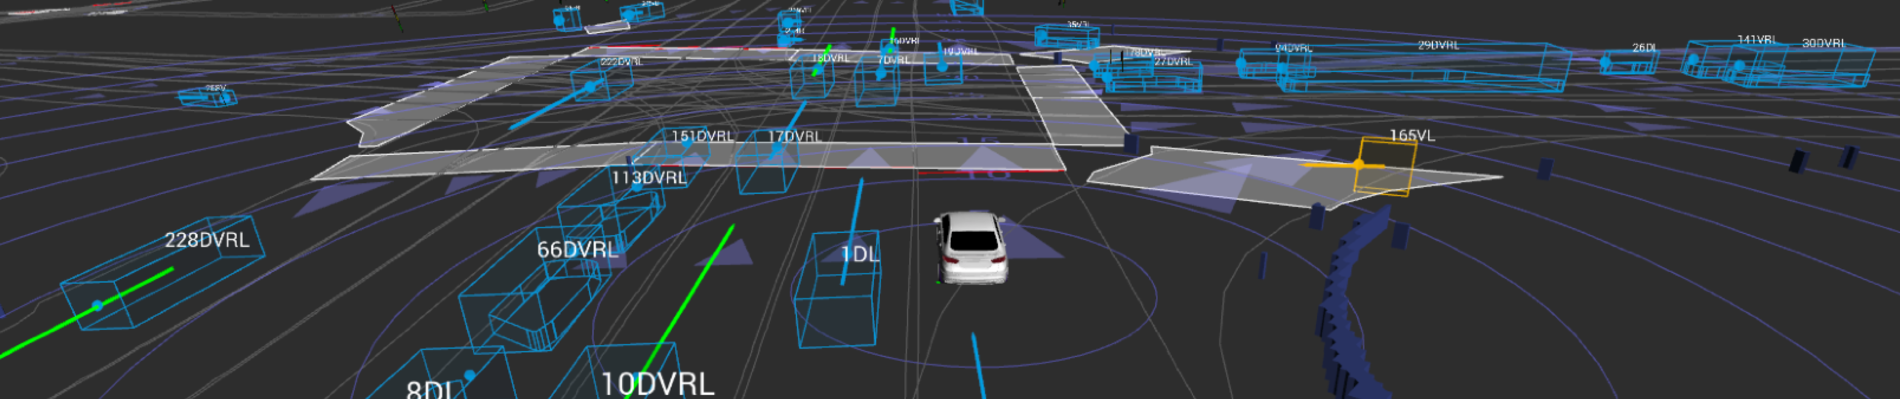
\includegraphics[width=0.9\textwidth]{images/lyft-hd-map.png}
  \caption{\textit{HD} мапа - \textit{Kaggle Lyft} \cite{kaggle_lyft} \label{kaggle-lyft-example}}
\end{figure}

На слици \ref{kaggle-lyft-example} се види пример визуализоване \textit{HD} мапе. Бело возило је агент, а плави правоугаоници су суседи. 
Са слике се види да мапе садрже и полигоне пешачких прелаза и још неке додатне податке. Подаци ових мапа су често у \textit{3D} формату
тј. узима се у обзир и висина. У реалном времену се ови подаци могу комбиновати са улазима из камера. 

\textcolor{orange}{\section{Циљ рада}}

Циљ овог рада је анализа различитих приступа разумевања контекста сцена у саобраћају. 
Под контекстом се подразумева разумевање статичког дела сцене који обухвата путеве,
семафоре, пешачке прелазе и слично, динамичког дела сцене који обухвата историју кретања објеката на сцени, и интеракције 
свих елеманата у том окружењу. 

Сцене се посматрају из птичје перспективе
и дате су у формату \textit{HD} мапа. На основу информација добијених из обрађених мапа и историје трајекторије објеката
на сцени се врши предвиђање трајекторија агената. Посебна пажња се посвећује анализи већ постојећих
техника заснованих на растеризацији сцена и графовских техника које захтевају трансформацију података у структуру графа. 
Главна инспирација су хијеархијска графовска неуронска мрежа \textit{VectorNet} \cite{vectornet} и \textit{HOME} \cite{home}
архитектура која претежно заснована на примени конволутивних мрежа над растеризованим подацима. 

Подаци једног сценарија (једна инстанца \textit{HD} мапе\textcolor{orange}{, један случај}) нису нужно дати само у једном облику 
тј. само једној структури. Историја
трајекторија може да се чува у табеларном формату, где се за сваки ред чува временски тренутак, идентификатор агента и координате
тог агента у том тренутку. Возно подручје може да буде задато као бинарна матрица где 1 означава да је могућа вожња на тој координати, 
а 0 да није могућа вожња. Први корак
сваке технике подразумева комбиновање и трансформацију података у одговарајући облик, било да је крајњи резултат слика или граф. У раду
се презентују детаљи имплементације припреме података у одговарајуће облике. 
Методе које се анализирају не нуде отворену имплементацију отвореног кода и не залазе у конкретне детаље имплементације. 

Квалитет модела зависи од начина на који се примењује доменско знање. Одређене кључне информације
са сцене могу да се изведу детерминистичким алгоритмима заснованим на одговарајућим хеуристикама. У раду се презентују
једноставне хеуристике које комбинују доменско знање са моделима машинског учења.


\chapter{Преглед основних градивних елемената}
\label{chp:razrada}

\section{Неуронске мреже}

TODO: Osnovno, MLP

\section{Конволутивне неуронске мреже}

TODO: CNN, Transposed CNN

\section{Графовске неуронске мреже}

TODO: Osnovno, opšte, GCN, GraphSage

\section{Механизам пажње}

TODO: attention

\textcolor{red}{\chapter{Преглед постојећих приступа}}
\label{chp:razrada}
% ------------------------------------------------------------------------------

\textcolor{red}{Уколико имамо више објеката на сцени за које треба да се изврши предвиђање трајекторија, онда је лакше да се предвиђање сваке 
трајекторије изврши из угла конкретног објекта. Тај објекат наставку реферише као агент. Сваки агент може да има свој референтни систем
и одговарајуће окружење у том систему тј. елементе сцене у околини тог агента. Скуп релеватних елемената као што су путеви, остала возила, пешаци и слично се
разликују од окружења једног агента до другог. Један од главних фактора за релеватност елемената је удаљеност тог елемента у окружењу од агента.}

\textcolor{red}{Предвиђање може да се извршава у једном кораку, где излаз модела подразумева више трајекторија (по једна трајекторија за сваког агента), 
или итеративно за сваког агента посебно. Сам приступ зависи од конкретног модела, 
али углавном су модели ограничени да итеративно генеришу предикције за сваког агента, што може да буде рачунски захтевније. 
Посматрано из угла аутономне вожње, скоро увек је интересантан само један агент на сцени који одговара возилу којим се управља.}

Технике за предикцију трајекторија више објеката могу да се групишу грубо у четири групе:
\begin{itemize}
  \item Технике прилагођене репрезентацијама временских серија;
  \item Технике засноване на растеризацији;
  \item Технике засноване на графовским репрезентацијама;
  \item Хибридне технике.
\end{itemize}

\textcolor{red}{У наставку ове главе биће укратко описане претходно наведене технике}

\section{Технике прилагођене репрезентацијама временских серија}

\textcolor{red}{Из поставке проблема може да се закључи да овај проблем може да се сведе на предвиђање временских серија, јер свака 
трајекторија може да се представи помоћу временских серија. У том случају је интуитиван иницијални приступ да се користе рекурентне неуронске мреже 
(\textit{eng. RNN - Recurrent Neural Network}) и конволутивне мреже за једнодимензионе сигнале} (\textit{CNN - Convolutional Neural Network}). 
Често коришћена \textit{LSTM} архитектура рекурентних неуронских мрежа \textcolor{red}{је} погодна за кодирање динамике објеката на сцени. 
\textcolor{red}{Динамика објеката се односи на историју трајекторија агента и осталих објеката на сцени.} 
\textcolor{red}{У случајевима када трајекторија једног објекта зависи од трајекторија осталих објеката, није довољно да се само узима у обзир
историја трајекторије агента. У том случају је погодно} да се користи механизам пажње као компонента модела која учи 
\textcolor{orange}{релевантне} везе између различитих објеката на сцени \cite{argoverse, social_lstm, attention_is_all_you_need}. 

\textcolor{red}{Један од главних проблема претходних приступа је неспособност модела да научи мултимодалну природу трајекторија на сцени. На слици
је \ref{multimodal-example} је приказан пример сценарија где не постоји само једна валидна предикција трајекторије. 
Ради успешног краткорочног планирања у аутономној вожњи, морају да се узму у обзир скоро сва могућа будућа стања сценарија. Модели
који као излаз дају само највероватнију трајекторију нису увек довољни. Бољи приступ је да се уместо модела који као излаз има највероватнију трајекторију користи
модел који као излаз има $N\ (N > 1)$ трајекторија заједно са вероватноћом сваке од тих трајекторија. Модели који се узимају у обзир у овом раду функционишу
по том принципу. }

\begin{figure}[H]
  \centering
  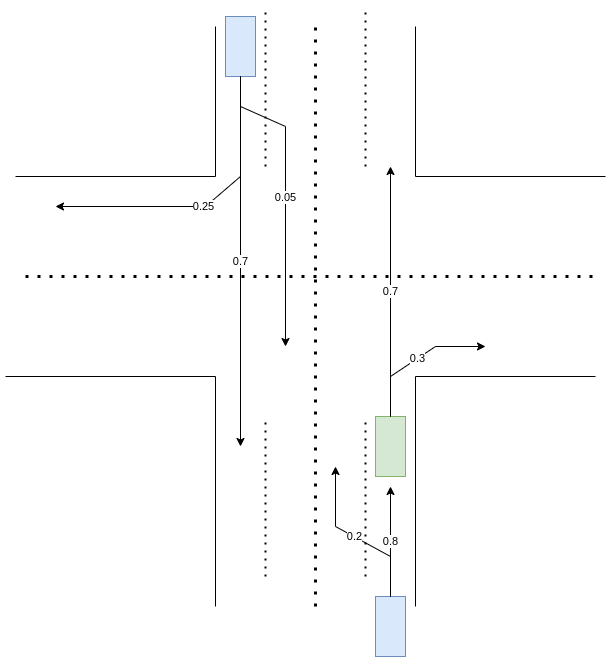
\includegraphics[width=0.5\textwidth]{images/multimodal.drawio.png}
  \caption{\textcolor{orange}{Милтимодална природа могућих будућих трајекторија - бројеви на трајекторијама представљају вероватноће}}
  \label{multimodal-example}
\end{figure}

\textcolor{red}{Битно је нагласити да трансформација модела који као излаз има једну трајекторију у модел који као излаз има више трајекторија није тако једноставно.
Природан избор за функцију грешке током тренирања је одступање предвиђене трајекторије од истините трајекторије. Конкретан пример
функције грешке је просечно еуклидско растојање тачака предвиђене трајекторије и истините трајекторије које одговарају истом временском тренутку. Ако
се тренира модел који предвиђа једну трајекторију са овом функцијом грешке (под претпоставком да квалитет и квантитет података нису проблем), 
онда ће он научити да предвиђа просечну трајекторију. Уколико се повећа број трајекторија у излазу модела, а функција грешке остане иста тј. предвиђене
трајекторије се упоређују са једном истинитом трајекторијм у сваком сценарију, то не значи да ће модел научити да узима у обзир и остале
вероватне трајекторије, већ ће вероватно генерисати само \textit{N} ,,дупликата`` трајекторија, где је \textit{N} број трајекторија у излазу 
тог модела. Овај проблем се назива колапс мода \textit{eng. mode collapse} и односи се на проблем игнорисања неких мода приликом генерисања предикција 
\cite{overcoming_mode_collapse}.}

Уместо учења модела који дају предикције трајекторија које \textcolor{red}{су} у просеку најбоље у тим случајевима, 
алтернатива је скуп модела заснованих на \textcolor{red}{условним} генеративним моделима који
омогућавају генерисање произвољног броја трајекторија кроз узорковање из \textcolor{red}{условне} расподеле 
(расподела је условљена историјом трајекторије, као и окружењем у којем се тај објекат налази). \textcolor{red}{Овакви модели нису имуни на колапс мода,
али боље превазилазе тај изазов.}
Пример \textcolor{orange}{таквог модела} је \textit{Social GAN} \cite{social_gan} архитектура која узима у обзир претходно наведене услове и генерише ,,социјално прихватљиве`` 
трајекторије пешака. \textcolor{red}{Током процеса предвиђања генеративни модели захтевају напредније алгоритме узорковања над великим бројем генерисаних
трајекторија ради оптимизације покривености трајекторијама тј. ради оптимизација 
односа будућих стања сценарија који је модел узео у обзир и свих могућих будућих стања сценарија. Чак и са одговарајућим алгоритмима,
није гарантована оптимална покривеност због стохастичког узорковања из латентног простора \cite{tnt}. Овакви модели могу да се користе
у аутономној вожњи, али су ипак погоднији за
проблем предвиђања трајекторија пешака у произвољном окружењу који није нужно улица, већ може на пример да буде и парк који има слабија ограничења
на кретање тог пешака.}

\section{Технике засноване на растеризацији}

Растеризација подразумева трансформацију \textit{HD} мапа у слике, где слике приказују сцене из птичје 
перспективе (\textit{eng. BEV - Bird's-eye-view}). \textcolor{orange}{То значи да различите структуре података које описују један сценарио 
морају да се конвертују у облик слике. На пример, историја трајекторија која је углавном задата у табеларном формату мора да се конвертује 
у слику или да се на неки начин комбинује са растеризованим подацима у оквиру архитектуре модела.}
Предност \textcolor{red}{слика} је могућност разумевања \textcolor{red}{интеракција елемената на мапи} 
коришћењем \textcolor{orange}{низа} слојева конволутивних неуронских мрежа.
\textcolor{red}{Идеја низа конволутивних мрежа је да преводу сирове слике у компактнији облик својстава који углавном има мању резолуцију, 
али већи број канала. Овако добијена својства се користе за предвиђање трајекторија.}
Конволутивне мреже нису ограничене да раде са RGB и сличним форматима слика. Сваком пикселу може да се додели \textcolor{orange}{вектор} својстава. 
Нека од очигледнијих својстава су: да ли агент заузима тај пиксел, да ли сусед (неагент) заузима тај пиксел,
да ли пиксел припада улици, ... Излаз CNN енкодера се углавном накнадно комбинује са осталим компонентама за генерисање резултата. 

Излази модела такође могу да се представљају као топлотне мапе \textcolor{red}{\textit{(eng. heatmap)}}. \textcolor{orange}{Структура топлотних мапа
одговара слици}, где се сваком пикселу додељује вероватноћа
да се агент налази на тој локацији. \textcolor{red}{За добијање топлотних мапа се користи енкодер-декодер архитектура, где се сирова слика
прво пресликава у компактнији облик својстава низом конволутивних мрежа (енкодер), а онда се 
применом низа транспонованих конволутивних слојева (декодер), које неформално представљају инверз конволутивних слојева, добија
топлотна мапа која је исте резолуције или редуковане резолуције у односу на улазну слику.
Како крајњи резултат треба да буде једна или више предикција трајекторија, неопходно је да се примени одговарајући алгоритам за
узорковање циљних тачака. Циљна тачка
се дефинише као последња локација предикције трајекторије. Главна мотивација за узорковање циљних тачака је претпоставка да уколико је познато где се
трајекторија завршава, онда је лако да се одреди цела та трајекторија тј. естимира кретање агента до крајње тачке}\footnote{\textcolor{red}{Претпоствка важи 
у случају када је агент возило које у саобраћају има ограничено кретање, док у случају човека који се креће у неком парку то није толико реална
претпоставка}}. \textcolor{red}{Број узоркованих крајњих тачака зависи од алгоритма и може да буде фиксан или да варира од једног до другог сценарија. 
Пример алгоритма је узорковање N циљних тачака тако да површина које њихове околине покривају има највећу сумарну вредност вероватноћа 
пиксела топлотне мапе. Околина
тачке може да буде круг са фиксном величином полупречника који представља параметар алгоритма узорковања. Када је позната циљна тачка трајекторије,
онда може да се користи једноставнији модели неуронских мрежа (нпр. потпуно повезане мреже) \cite{home, centernet}.}

Архитектура \textit{HOME} \cite{home} користи принцип за паралелно кодирање растеризоване сцене \textcolor{orange}{(статички део)} 
и трајекторија oбјеката \textcolor{orange}{(динамички део)}. Резултати
\textcolor{orange}{статичког и динамичког дела модела} се спајају \textcolor{orange}{конкатенацијом} и прослеђују као улаз у декодер за генерисање топлотне мапе. 
Узорковањем тачака из топлотних мапа се добија скуп \textcolor{orange}{циљних} тачака. \textcolor{orange}{Различити алгоритми узорковања дају
боље перформансе модела по различитим метрикама за евалуацију квалитета трајекторија у аутономној вожњи. Независно од модела топлотне мапе
се тренира модел који естимира кретање трајекторије када је позната њена крајња тачка.}

Могуће је растеризовати потпуно податке тј. растеризовати и трајекторије као низ слика. Свака слика садржи скуп тачака које представљају
локације објеката. Архитектура \textit{CASPNet} \cite{caspnet} примењује CNN енкодер на свако стање \textcolor{orange}{историје сценарија} 
и користи ConvLSTM \cite{convlstm} \textcolor{orange}{модел} за разумевање
темпоралних веза \textcolor{orange}{тих слика}. На овај начин се \textcolor{orange}{добијају} својства динамичког дела сцена. 
На сличан начин је могуће и извући својства и за 
статички део (возне линије, возни површине, ...) користећи класичне конволутивне мреже. Комбинацијом ових података се генеришу
трајекторије које су исто \textcolor{orange}{дате} у растеризованом облику. \textcolor{orange}{Овакав приступ је рачунски веома скуп.}

\section{Технике засноване на графовским репрезентацијама}

Мапе имају комплексну топологију\textcolor{orange}{, а технике} засноване на растеризацији користе конволуцију која тешко 
извлачи потпуно семантику тих мапа. \textcolor{red}{Taкође, конволуција је скупа операција}. Алтернатива је моделовање мапа графовским структурама. 
Технике засноване на графовском репрезентацијом као улаз добијају стање мапе кодиране као граф и примењују моделе графовских неуронских мрежа. 
Две архитектуре које представљају основе за већину архитектура ове групе су \textit{LaneGCN} \cite{lanegcn} и \textit{VectorNet} \cite{vectornet}.

Мапа може да се моделује као скуп повезаних сложених линија (\textit{eng. polylines}), где сваком објекту одговара једна усмерена сложена линија. 
\textit{VectorNet} је хијерархијска графовска неуронска мрежа која као улаз добија мапу која је моделована као скуп 
сложених линија, а као резултат даје \textcolor{orange}{предикцију једне трајекторије за сваког агента}.\footnote{\textcolor{orange}{У овом контексту се издвајају агенти
као објекти на сцени за које се врши предвиђање трајекторије.}} Идеја је да се прво извуку својста из сложених 
линија појединачних објеката, а онда пронађу одговарајуће међусобне везе између објеката и везе између објеката и возних линија. 
За проналазак међусобних веза се користи механизам пажње \cite{attention_is_all_you_need, vectornet}.
\textcolor{red}{Мотивација је следећа: Нису сви објекти у околини значајни за конкретног агента,
јер они објекти који су далеко од њега и иду супротном линијом не утичу толико на његово кретање. Нису ни сви путни сегменти значајни за агента.
Свакако су значајни путни сегменти који се поклапају са историјом трајекторије агента и путни сегменти по којим агент може потенцијално да се креће
у скоријој будућности. Задатак модела је да закључи који елементи сцене су значајни.}

Архитектура \textit{LaneGCN} нуди варијанту конволутивних графовских мрежа (\textit{GCN - Graph Convolution Network}) \textcolor{orange}{\cite{gcn}}
која је специјализована за графове путних \textcolor{orange}{сегмената} које имају различите типове веза. Користе се различите матрице
повезаности за суседе, претходнике, следбенике (леви и десни) у контексту \textcolor{orange}{путних сегмената}. 
За сваку матрицу повезаности може да се примени класичан GCN, а
комбиновањем тих елемената је добија један \textit{LaneGCN} слој \cite{lanegcn}. Сам модел се своди на \textit{GCN} са више матрица повезаности.

\section{Хибридне технике}

Хибридне технике користе комбинацију структура графова и BEV слика. \textcolor{red}{Модел \textit{GOHOME} је модификована верзија \textit{HOME} 
модела који уместо CNN енкодера и растеризоване слике као улазне податке, користи \textit{LaneGCN} архитектуру као енкодер и податке
у облику графа}. Заправо ансамбл ова два модела \textit{HOME} и \textcolor{red}{\textit{GOHOME}}
даје најбоље резултате по \textit{MR} метрици. \footnote{Објашњење за ову метрике се налази у секцији \textcolor{red}{о евалуацији}}

\section{Технике засноване на облацима тачака}

Последња група нешто одступа од осталих \textcolor{red}{по броју објављених радова}, 
али и даље даје добре резултате. Подаци се посматрају као облаци тачака (\textit{eng. point cloud}) 
и примењују се технике намењене за такву структуру података. Основна
архитектура је \textit{TPCN} \cite{tpcn} која је заснована на \textit{PointNet} \cite{pointnet}. \textcolor{red}{Већина осталих техника су ,,изведене`` из ње}.

% ------------------------------------------------------------------------------
% ------------------------------------------------------------------------------

\chapter{Метрике за евалуацију модела}
\label{chp:razrada}
% ------------------------------------------------------------------------------

Неке од стандардних метрика за евалуацију квалитета предикције трајекторија су ,,просечнa грешка одступања`` (\textit{eng. ADE - Average Displacement Error})
и ,,грешка последњег одступања`` (\textit{eng. FDE - Final Displacement Error}). У наставку се користе енглеске скраћенице \textit{ADE} и
\textit{FDE}. Метрика \textit{ADE} се рачуна као просечно еуклидско растојање између тачака предикције и истините трајекторије у свим
временским тренуцима који одговарају тој трајекторији. 
Метрика \textit{FDE} узима у обзир само последњу тачку тј. еуклидско растојање између последње тачке реализације и предикције.
Што су метрике \textit{ADE} и \textit{FDE} мање након евалуације модела, то је модел квалитетнији. \cite{social_gan, argoverse}.  
У наставку се налазе формуле у случају да се посматра тачно један објекат (нпр. само агент):

\begin{figure}[H]
  \centering
  $ADE = \frac{1}{T}\sum_{k=1}^{T}\sqrt{(x_k - \hat{x}_k)^2 + (y_k - \hat{y}_k)^2}$
\end{figure}

\begin{figure}[H]
  \centering
  $FDE = \sqrt{(x_{last} - \hat{x}_{last})^2 + (y_{last} - \hat{y}_{last})^2}$
\end{figure}

Метрике се једноставно уопштавају у случајевима где постоји више објеката на сцени:

\begin{figure}[H]
  \centering
  $ADE = \frac{1}{T\times N}\sum_{n=1}^{N}\sum_{k=1}^{T}\sqrt{(x^n_k - \hat{x}^n_k)^2 + (y^n_k - \hat{y}^n_k)^2}$
\end{figure}

\begin{figure}[H]
  \centering
  $FDE = \frac{1}{N}\sum_{n=1}^{N}\sqrt{(x^n_{last} - \hat{x}^n_{last})^2 + (y^n_{last} - \hat{y}^n_{last})^2}$
\end{figure}

Ако узмемо у обзир претпоставку да се релативно детерминистички може одредити трајекторија ако је дата њена последња тачка 
(што је у случају возила у сабраћају разумна претпоставка), онда су ове две метрике корелисане у смислу да модел 
који има добар \textit{FDE}, има и добар \textit{ADE} (и супротно).

Ове једноставне метрике су погодне под претпоставком да је расподела трајекторија унимодална у односу на дату историју тј. да за сваку историју трајекторије 
постији тачно једна смислена предикција. 
Скупови података трајекторија могу да имају јачу стохастичку природу због природе самог проблема или због непотпуних информација о окружењу.
Пример таквог скупа података је скуп трајекторија пешака. Пешак који је прешао пешачки прелаз, може у том тренутку да скрене лево или десно.
У том случају имају два вероватна сценарија за исту историју трајекторије, али углавном немамо информације о циљевима самог пешака \cite{social_gan, best_of_many_cvae}. 
У случају возила је ситуација мало блажа због већег броја ограничења, али проблем и даље постоји. На слици \ref{multimodal-example} је већ приказан пример једног 
таквог сценарија у саобраћају.

Скуп ,,најбољи из групе`` (\textit{eng. ,,Best of Many``}) метрика узимају у обзир мултимодалну природу расподела трајекторија. Модел може
да генерише неколико различитих предикција трајекторија и да за сваку трајекторију да одговарајућу вероватноћу (поузданост). За рачунање грешке 
се узима предикција која је најбоља по дефинисаном критеријуму. Критеријум не мора да се поклапа са самом мером која се користи 
тј. не мора нужно да се изабере трајекторија која је најбоља по тој мери, већ за тај избор може да се користи друга мера. \cite{best_of_many_cvae, argoverse}. 
Претходно наведене метрике \textit{ADE} и \textit{FDE} се уопштавају у \textit{minADE} и \textit{minFDE}. Због једноставности узимају се у обзир облици
са једним објектом: \cite{Disdis, best_of_many_cvae}

\begin{figure}[H]
  \centering
  $minADE = ADE(\displaystyle\argmin_{\hat{A}_k} FDE(\hat{A}_k, A), A), k \in \{1, ..., K\}$ 
\end{figure}

\begin{figure}[H]
  \centering
  $minFDE = \displaystyle\min FDE(\hat{A}_k, A), k \in \{1, ..., K\}$
\end{figure}

Овде је $A_k$ истинита трајекторија, а $\hat{A}_k$ трајекторија из скупа предикција. Обе метрике \textit{minFDE} и \textit{minADE} 
се своде на избор трајекторије која најмање одступа од истините трајекторије у последњем тренутку тј. бира се трајекторија која има најмањи \textit{FDE}.

Уколико модел генерише више од \textit{K} трајекторија, узима се и обзир првих \textit{K} по поузданости. У специјалном случају када је $K = 1$, онда 
\textit{minFDE} постаје \textit{FDE}, a \textit{minADE} постаје \textit{ADE}. 
Проблем са \textit{minADE} i \textit{minFDE} је у томе што не узимају у обзир остале трајекторије поред најбоље и самим тим се не прави разлика
између предикције са свим добрим трајекторијама и предикције са једном добром трајекторијом \cite{Disdis}. 
Друга замерка овим метрикама је што не узимају у обзир поузданост предикција након филтрирања \textit{K} трајекторија. Уколико је најбоља трајекторија
прецизна, желимо и даље да знамо да ли је модел сигуран или је добар резултат последица ,,среће``. Модификоване метрике \cite{home}: 

\begin{figure}[H]
  \centering
  $p\mbox{--}minADE = ADE(\hat{A}_{min}, A) - \ln{P(\hat{A}_{min}|E)}$
\end{figure}

\begin{figure}[H]
  \centering
  $p\mbox{--}minFDE_{prob} = FDE(\hat{A}_{min}, A) - \ln{P(\hat{A}_{min}|E)}$
\end{figure}

Овде је $\hat{A}_{min}$ трајекторија која има најбољу $FDE$ оцену, а $p(\hat{A}_{min}|E)$ је условна вероватноћа те 
трајекторије $\hat{A}_{min}$ у односу на стање окружења $E$. Уколико је мала грешка по метрици \textit{ADE} (\textit{FDE}) за одговарајућу трајекторију, 
али њена вероватноћа има малу вредност, онда негативан логаритам те вероватноће има велику вредност \cite{argoverse}.
У импементацији се ова вероватноћа ограничава са доње стране, како не
би дошло до прекорачења због велике апсолутне вредности након примене логаритма на веома мале вредности.

Уместо упросечавања \textit{L2} растојања у сваком кораку, могу да се броје кораци у којима трајекторије одступају за више од 
дозвољеног оступања $MR_{thresh}$ (\textit{miss rate threshold}). 
Мотивација за ову метрику је чињеница да одступање које је 1 или 2 метра од реализације није толико релевантно у односу на одстпуање од 
неколико метара \cite{home}. Такође постоји верзија метрике која узима у обзир вероватноћу и кажњава предикцију 
модела ако је добра, а модел је ипак несигуран.

\begin{figure}[H]
  \centering
  $MR = \sum^T_{k=1} I(||\hat{A}^{k} - A||_{2} \geq MR_{thresh})$
\end{figure}

\begin{figure}[H]
  \centering
  $MR_{prob} = \sum^T_{k=1} I(||\hat{A}_{k} - A||_{2} \geq MR_{thresh}) + I(||\hat{A}_{k} - A||_{2} < MR_{thresh}) \cdot (1.0 - P(\hat{A}^{k}|E))$
\end{figure}

Обична $MR$ метрика рачуна само број тачака трајекторије које одступају много од одговарајуће тачке истините трајекотрије, док
$MR_{prob}$ додатно кажњава ситуације у којима не постоји велико одступање, али модел није довољно сигуран. 
У случају \textit{Argoverse} скупа података, за параметар $MR_{thresh}$ се узима 4 пиксела тј. 2 метра у реалном свету. 

Све до сада наведене метрике су опште примене на било које објекте за које се предвиђају трајекторије. Пошто је агент углавном возило, може да
се анализира да ли предвиђена трајекторија скреће са пута. Због тога се уводи метрика ,,сагланост са возним подручјем`` 
(\textit{eng. DAC - Drivable Area Compilance}), која одређује учесталост трајекторија које нису скренуле са пута од изабраних 
\textit{K} трајекторија \cite{argoverse}:

\begin{figure}[H]
  \centering
  $DAC = \frac{DAC_{occurences}}{T}$
\end{figure}

У евалуацији модела се узимају у обзир све метрике. За параметар \textit{K} за \textit{minADE} и \textit{minFDE} се узима вредност 6.

\chapter{Припрема података \label{initprep}}

Основни скуп података за тренирање и тестирање техника предвиђања трајекторија је \textit{Argoverse Motion Forecasting} скуп података
који се састоји од 324 хиљаде сценарија у саобраћају сачиуваних као \textit{HD} мапе. Постоје две групе \textit{HD} мапа
за градове Питсбург и Мајами. Коришћењем аутономних возила су генерисани сценарији који представљају неколико узастопних слика сцена (у табеларном формату)
на деловима мапа. Сви детаљи о овом скупу података се могу пронаћи на адреси 
\href{https://www.argoverse.org/index.html}{\color{blue}{www.argoverse.org}} \cite{argoverse}. \\


\noindent Kључне информације које се издвајају из сваког сценарију су:
\begin{itemize}
  \item Мапа сценарија (Питсбург или Мајами);
  \item Трајекторије агената;
  \item Трајекторије осталих објеката на сцени (суседи);
  \item Путни сегменти.
\end{itemize}

У наставку се описује процес прве фазе припреме података. Формат података који се добија након ове фазе је погодан
за даљу трансформацију у графовску структуру или слику (растеризован облик).

\section{\textit{Argoverse} интерфејс}

Сирови подаци сваког сценарија се векторизују и чувају у полу-структуираном формату. 
За парсирање и обраду улазних података се користи \textit{argoverse API} интерфејс. Сваки град се састоји из скупа
повезаних путних сегмената који чине један усмерен граф. Функције које се користе из \textit{Argoverse} интерфејса се 
односе на операције над тим графом. Скуп функција које се користе:
\begin{itemize}
  \item Одређивање свих путних сегмената који се налазе у околини агента на основу последње тачке у историји трајекторије.
  \item Одређивање следбеника, претходника и суседа у графу у односу на посматрани путни сегмент.
  \item Читање метаподатака о путним сегментима: Да ли се путни сегмент налази у неком пресеку, да ли постоји контрола саобраћаја и
        да ли је путни сегмент усмерен лево, десно или је прав.
  \item Примена претраге у дубину над графом у односу на посматрани путни сегмент који представља почетни чвор у алгоритму претраге.
  \item Одређивање путног подручја града (матрица).
\end{itemize}

Циљ овог корака процесирања података је векторизација података у формат који је је независан од модела који се користи тј.
обједињавање заједничког дела припреме података.

\section{Припрема трајекторије агента}

Трајекторија агента\footnote{Низ $(x, y)$ тачака, где је приближна временска разлика између две тачке око 0.1 секунди у \textit{Argoverse}
скупу података.} 
се дели на два дела: историја (својства) и реализација (будуће вредности). Реализација се састоји од $N_r$ вредности
$x$ и $y$ координата тј. облик реализације је $(N_r, 2)$.
Историја се аналогно формира да садржи историју $N_h$ опажања $x$ i $y$ координата. Овај део трајекторије иде непосредно
пре реализације. Посматрамо следеће случајеве:
\begin{itemize}
  \item Постоји више од $N_h + N_r$ опажања: Одбацује се реп трајекторије (првих неколико вредности хронолошки гледано);
  \item Постоји мање од $N_{hmin} + N_r$ опажања: Сценарио се одбацује (сматра се да је невалидан);
  \item Постоји између $N_{hmin} + N_r$ и $N_h + N_r$ опажања: реп трајекторије који се односи на историју трајекторије 
        се допуњава до димензије $N_h + N_r$ посматрано као да објекат мирује у тим тренуцима.
\end{itemize}
Овде је $N_{hmin}$ минимални број опажања у историји трајекторије неопходан за вршење предвиђања трајекторија. Уколико је историја
трајекторије скоро потпуно непозната, онда није реално да се очекују добре перформансе модела на том сценарију. Филтрирање се
односи на скуп података за учење, а током предвиђања је свакако неопходно да се да неки резултат. Параметар $N_r$ је постављен на \textit{30},
а $N_h$ је постављен на \textit{20}. Ове вредности су изабране тако ради усаглашавања са осталим радовима. Параметар $N_{hmin}$ је
постављен на \textit{5}, али избор вредности је флексибилан. 
Коначно, облик историје је $(N_h, 3)$, где трећа вредност означава да ли је опажање право ($1$) или допуњено ($0$).

Све координате се нормализују тако да су релативне у односу на последње опажање историје агента. Последње опажање историје
агента има координату (0, 0) у новом координатном систему, а све остале тачке се транслирају за вектор $-C$, где је $C$ оригинална позиција
последњег опажања. Координатни систем се такође ротира тако да се вектор који је одређен првом и последњом тачком историје трајекторије,
што чини наивно апроксимиран правац трајекторије, поклапа са \textit{y}-осом сличко као и у оригиналном \textit{Vectornet} раду \cite{vectornet}. Последња
трансформација је скалирање свих координата са $\frac{1}{25}$, где је ова вредност добијена анализом стандардних девијација свих тачака
на сценаријима (узета је просечна вредност свих сценарија). Ове трансформације су кључне за перформансе модела, јер је сам проблем који се решава
једноставнији:
\begin{itemize}
  \item Применом транслације модел не мора да учи где се агент налази, јер је то увек (0, 0) координата;
  \item Применом ротације моделу је олакшано учење усмерења трајекторије тј. моделу је лакше да одреди оријентацију агента;
  \item Применом скалирања се добијају стабилнији градијенти.
\end{itemize}
Оригинална позиција последњег опажања и угао ротирања се чувају за сваки сценарио. На овај начин је могуће извршити
инверзно пресликавање у оригинални координатни систем. За све метрике наведене у претходој секцији сем \textit{DAC} је довољно
да се само изврши инверзно скалирање, јер су транслација и ротација изометрије које чувају растојања. За метрику \textit{DAC} је 
неопходно да се изврши усклађивање са мапом путног подручја.

\section{Припрема трајекторија суседа}

Трајекторије суседних објеката се деле на два дела аналогно трајекторији агента. Неопходно је да се синхронизују трајекторије 
суседних објеката по временским ознакама (eng. \textit{timestamp}) са трајекторијом агента, јер не постоји у сваком тренутку исти
број објеката на сцени. Након синхронизације се трајекторије деле на историју и реализацију и проверава се да ли дужине тих
делова задовољавају критеријуме:
\begin{itemize}
  \item Уколико је дужина трајекторије историје краћа од $N_{homin}$, онда се објекат одбацује;
  \item Уколико је дужина трајекторије реализације краћа од $N_{romin}$, онда се објекат исто одбацује.
\end{itemize}
Вредности параметара $N_{homin}$ и $N_{romin}$ се постављају на \textit{5} и \textit{3}.

Као додатна провера, за сваки сусед се провера растојање од агента. Уколико је сусед превише далеко, онда се се он одбацује.
Критеријум за одбацивање суседа узима у обзир брзину агента (по $x$ и $y$ оси одвојено) и растојање њихових последњих опажања
у трајекторији историје. Уколико неки од следећих услова није
испуњен, онда се сусед игнорише у сценарију: 
\begin{itemize}
  \item $\frac{O_n^x}{V_s^x} \leq T_{steps}$
  \item $\frac{O_n^y}{V_s^y} \leq T_{steps}$
\end{itemize}
где је $O_n^x$ ($O_n^y$) нормализована $x$ ($y$) координата суседа, $V_s^x$ ($V_s^y$) је наивно 
апроксимирана брзина агента
по $x$ ($y$) оси\footnote{Брзина се апроксимира као просек промена координата у трајекторији историје} и $T_{steps}$ је параметар толеранције.
Трајекторије се секу или допуњавају до фиксног облика (kao што је то у случају припреме трајекторије агента). 
Векторизован облик: $(N_n, N_h, 3)$ за историје трајекторија и $(N_n, N_r, 3)$ за реализацију трајекторија, где је $N_n$ број судедних објеката. 
Трећа вредност је информација о томе да ли је та тачка допуњена или не.

\section{Припрема путних сегмената}

На основу локације агента се издвајају путни сегменти који су у околини агента са радијусом $D_{lsinit}$ по \textit{L1} растојању. Уколико нема
пронађених сегмената централних линија, онда се вредност за $D_{lsinit}$ множи са $K_{ls}$\footnote{$D_{lsinit}$ и $K_{ls}$ су фиксне вредности
у \textit{argoverse} интерфејсу} до највише $D_{lsmax}$. Ако и даље нема сегмената, 
онда се сценарио одбацује, јер није пронађен ниједан путни сегмент у околини. 
За сваки сегмент се чува низ од 20 $(x, y)$ координата приширених са метаподацима:
\begin{itemize} 
  \item \textit{is\_intersection} - да ли се сегмент сече са неким сегментом,
  \item \textit{turn\_right} - да ли је у питању скретање у десно, 
  \item \textit{turn\_left} - да ли је у питању скретање у лево, 
  \item \textit{turn\_none} - да ли нема стретања, 
  \item \textit{is\_traffic\_control} - да ли постоји контрола саобраћаја. 
\end{itemize}
Коначан облик је $(N_{ls}, 20, 7)$ тј. низ $N_{ls}$ путних сегмената дужине 20, где свака тачка путног сегмената има своје 2 координате
и 5 вредности за метаподатаке. 

\section{Припрема кандидата путних сегмената}

Постоји коначан број путних сегмената по којој
објекат може да се креће у скоријој будућности на задатој мапи. Због тога је корисно да се информације о кандидатима путних сегмената
користе као улаз у модел или као хеуристике.
\textit{Argoverse} интерфејс нуди своју имплементацију
за проналазак кандидата путних сегмената. Дат је поједностављен алгоритам \ref{argoverse-clcand} у \textit{Python} 
псеудокоду који описује укратко идеју алгоритма.

\begin{figure}
\begin{python}
def argoverse_algoritam(trajektorija, avm, dfs_radijus, min_duz, max_duz):
  # trajektorija: istorija trajektorije agenta 
  # avm: Argoverse mapa (interfejs ka grafu mape)
  # dfs_radijus: uslov zaustavljanja dfs algoritma
  # min_duz: Minimalna duzina poklapanja trajektorije i putnog segmenta
  # max_duz: Maksimalna duzina poklapanja trajekotrije i putnog segmenta

  prva_tacka = trajektorija[0]
  poslednja_tacka = trajektorija[-1]
  putni_segmenti = []  # trenutni putni segmenti
  radijus = 2  # trenutni radijus

  # radijus povecava dok se ne pronadju neki putni segmenti 
  # u okolini po L1 rastojanju (okolina je kvadrat)
  while len(putni_segmenti) == 0:
    putni_segmenti = avm.pronadji_putne_segmente_u_okolini(
      poslednja_tacka, radijus)
    radijus *= 2

  # Za svaki putni segment se pronalaze njegovi prethodnici
  # i sledbenici u grafu koji se onda objedinjuju 
  # (svaki prethodnik sa svakim sledbenikom)
  potpuni_putni_segmenti = []
  for ps in putni_segmenti:
    sledbenici = avm.dfs(ps, dfs_radijus)
    prethodnici = avm.dfs(ps, dfs_radijus, unazad=True)
    for p in prethodnici:
      for s in sledbenici:
        potpuni_putni_segmenti.append(objedini_segmente(p, s))

  # svi putni segmenti se aproksimiraju parametrizovanom krivom P(t)
  aproksimirani_putni_segmenti = aproksimacija_ps(potpuni_putni_segmenti)

  filtrirani_putni_segmenti = []
  # pronalaze se putni segmenti koji se najbolje poklapaju po duzini
  # sa istorijom trajektorije agenta
  for aps in aproksimirani_putni_segmenti:
    t_pocetak = aps.projekcija(prva_tacka)
    t_kraj = aps.projekcija(poslednja_tacka)
    duzina = t_kraj - t_pocetak
    if duzina >= min_duz and duzina <= max_duz:
      filtrirani_putni_segmenti.append(aps)
  return filtrirani_putni_segmenti
\end{python}
\caption{Поједностављен \textit{Argoverse} алгоритам за проналазак кандидата путних сегмената\label{argoverse-clcand}}
\end{figure}

Овај алгоритам у великом броју случајева погађа кандидате путних сегмената. У теорији је главна мана што узима у обзир само прву и последњу
тачку трајекторије агента. На слици \ref{argoverse-clcand-flaws} је направљен вештачки пример где алгоритам ради лоше. Нека је зелена стрелица
трајекторија агента и нека су плава и црвена стрелица путни сегменти који се узимају у обзир. Црвени путни сегмент је сличнији
трајекторији агента од плавог путног сегмента, али крајеви плавог путног сегмента и крајеви трајекторије агента се скоро савршено поклапају. 
То значи да се приоритет даје плавом сегменту иако је визуално више има смисла црвени путни сегмент.

\begin{figure}[H]
  \centering
  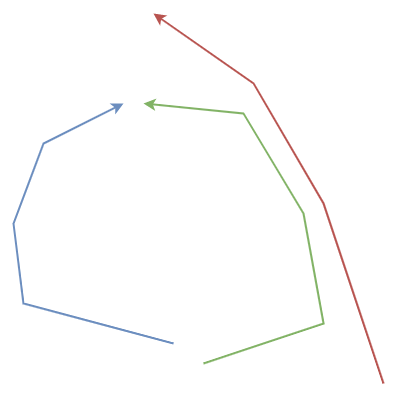
\includegraphics[width=0.5\textwidth]{images/argoverse-clcand-flaws.drawio.png}
  \caption{Пример где \textit{Argoverse} алгоритам за проналазак кандидата не даје тачне одговоре}
  \label{argoverse-clcand-flaws}
\end{figure}

Током тренирања \textit{VectorNet} модела који ће бити објашњен у наредној секцији, анализом података је примећено да је један од главних
разлога лошијих перформанси заправо слаб квалитет узорковања кандидата путних сегмената. Није ретко да се изабере путни сегмент који припада
супротној линији вожње и да због тога предикције буду јако лоше. Из тих разлога је одлучено да се имплементира једноставнији алгоритам
који се своди на коришћење \textit{DTW (Dynamic Time Warping)} методе и апроксимације угла између трајекторије и путног сегмента. приказан
је алгоритам \ref{dtw-algorithm} као \textit{Python} псеудокод.

\begin{figure}
  \begin{python}
  def dtw_algoritam(trajektorija, avm, dfs_radijus, putni_segmenti, 
      k = 3, max_ugao = 90):
    # trajektorija: istorija trajektorije agenta 
    # avm: Argoverse mapa (interfejs ka grafu mape)
    # dfs_radijus: uslov zaustavljanja dfs algoritma
    # putni_segmenti: koriste se putni segmenti dobijeni iz prethodnog koraka
    # k: broj najboljih putnih segmenata koji se uzimaju u obzir kao kandidati
    # max_ugao: Maksimalni ugao uzmedju trajektorije 
    #           i kandidata putnog segmenta
    
    # racuna se rastojanje putnog segmenta od trajektorije
    # koristi se dtw metoda sa L2 metrikom
    rastojanje_putni_segment = []
    for ps in putni_segmenti:
      rastojanje = dtw(trajektorija, ps)
      rastojanje_putni_segment.append((rastojanje, ps))

    # sortiranje po rastojanju
    rastojanje_putni_segment = sorted(rastojanje_putni_segment)
    # rastojanje vise nije bitno
    putni_segmenti = [ps for _, ps in rastojanje_putni_segment]
    putni_segmenti = putni_segmenti[:k]  # k najboljih

    # za svakog od putnih segmenata se pronalaze sledbenici dfs algoritmom
    kandidati = []
    for ps in putni_segmenti:
      sledbenici = avm.dfs(ps, dfs_radijus)
      kandidati.extend(sledbenici)

    kandidati = list(set(kandidati))  # uklanjanje duplikata

    # kandidati se filtriraju na osnovu ugla izmedju putnog segmenta
    # i trajektorije
    filtrirani_kandidati = []
    traj_pravac = izracunaj_pravac_trajektorije(trajektorija)
    traj_ugao = izracunaj_ugao_pravca(traj_pravac)
    for ps in kandidati:
      ps_pravac = izracunaj_pravac_trajektorije(ps)
      ps_ugao = izracunaj_ugao_pravca(ps_pravac)
      ugao = abs(traj_ugao - ps_ugao)
      if ugao > min_ugao:
        continue
      
      filtrirani_kandidati.append(ps)

    return filtrirani_kandidati

  \end{python}
  \caption{Алгоритам заснован на \textit{dtw} метрици и хеуристици угла између правца трајекторија \label{dtw-algorithm}}
  \end{figure}

Идеја је следећа: Уместо да се узима у обзир само последња тачка, упоређују се све тачке путног сегмента и трајекторије 
(путни сегмент је такође трајекторија). Коришћење \textit{ADE} метрике није идеално за поређење временских серија, јер 
то подразумева јака ограничења за асоцијације тачака. Асоцијација тачака се односи на то која тачка прве трајекторије може 
да се упари са којом тачком друге трајекторије. У случају \textit{ADE} метрике, свака тачка прве трајекторије
може да се упари само са једном тачком друге трајекторије. Метода \textit{DTW} одбацује то ограничење и омогућава
да свака тачка једне трајекторије може да се упари са било којом тачком друге трајекторије. Остају ограничења да једна
тачка једне трајекторије може да се упари са највише једном тачком друге трајекторије (а може и мање) и 
немогуће је испреплетано упаривање (ако се тачка 5 упари са тачком 8, онда тачка 4 не може да се упари са тачком 9). Метода
\textit{DTW} има разне примене над временским серијама, а алгоритам је уопштење Левештајновог растојања за ниске. На слици
\ref{euclidean_vs_dtw} се илуструје начин функционисања методе. У алгоритму се узима најбољих $K_c$ кандидата пре примене 
\textit{DFS}-a.

\begin{figure}[H]
  \centering
  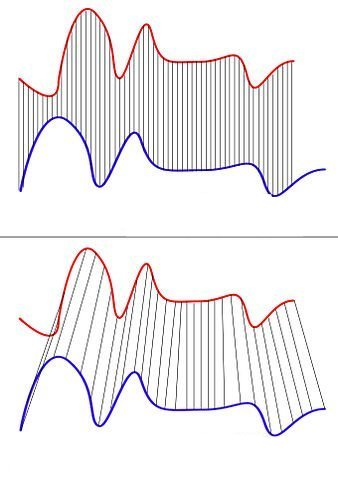
\includegraphics[width=0.5\textwidth]{images/Euclidean_vs_DTW.jpg}
  \caption{Упоређивање серија помоћу класичног еуклидског растојања (горе) и \textit{DTW} методе (доле)}
  \label{euclidean_vs_dtw}
\end{figure}

Упоређивање трајекторија на овај начин није довољно. Проблем прави трајекторија агента на сценама где се он не креће или се веома споро креће. Пошто
се \textit{DTW} своди на еуклидско растојање, онда у том случају може да се деси упаривање са најближим путним сегментом. Проблем код тога 
је што је путни сегмент одређен централном трајекторијом и ако агент није потпуно усклађен са његовим путним сегментом (нпр. искаче мало
из своје траке), онда је 
најближи путни сегмент заправо онај суседни који има супротну траку. Узимање путног сегмента са супротном траком је катастрофално,
јер применом \textit{DFS}-а се врши претрага у потпуно погрешном смеру. Због тога се додаје хеуристика која упоређује углове између
трајекторија кандидата путних сегмената добијених \textit{DTW} методом и угла трајекторије агента. Угао се одређује као угао вектора правца
трајекотрије, а вектор правца је одређен првом и последњом тачком трајекторије. Уколико је угао између трајекторије агента и 
трајекторије путног сегмента већи од $\theta_{min}$ степени, онда се тај путни сегмент одбацује. За $K_c$ се узима вредност 3, а
за $\theta_{min}$ се узима вредност 90.

Коначан векторизован облик је: $(N_c, N_r, 3)$, где је $N_c$ број пронађених кандидата,
$N_r$ дужина трајекторије реализације. Пошто се путеви допуњавају по потреби до димензије $N_r$, користи се трећа координата
за маску. 

\section{Преглед дефинисаних параметара}

На табели \ref{dp-params-table} се види преглед свих параметара процеса. Параметри $N_r$ и $N_h$ су изабрани тако да се поклапају
са осталим радовима. Ако би ти параметри били другачији, онда поређење метрика нема толико смисла. Остали параметри 
су изабрани интуицијом. Престпоставка је да претрагом параметара може да се повећа квалитет података за учење, а самим тим
и квалитет модела. Како је та опција рачунски јако скупа, у овом случају се прескаче. 

\begin{table}[H]
  \begin{tabular}{c|c}
    Ознака параметра & Објашњење \\
    \hline
    $N_r$ & Дужина трајекторије реализације (део који се предвиђа) \\
    $N_h$ & Дужина трајекторија историје \\
    $N_{hmin}$ & Минимална дужина трајекторије историје пре допуњавања \\
    $N_{hоmin}$ & Минимална дужина трајекторије историје суседа пре допуњавања \\
    $N_{rоmin}$ & Минимална дужина трајекторије реализације суседа пре допуњавања \\
    $T_{steps}$ & Умножак максималног растојања до сегмента пута \\
    $D_{lsmax}$ & Максимално растојање до пута \\
    $K_c$ & Број најбољих путних сегмената по \textit{DTW} методи \\
    $\theta_{min}$ & Најмањи угао између правца путног сегмента и правца трајекторије агента
  \end{tabular}
  \caption{Преглед параметара припреме података (TODO: proveriti da neki parametar nije preskocen)}
  \label{dp-params-table}
\end{table}

\section{Визуализација}

На сликама \ref{scenario-example-148229} и \ref{scenario-example-16518} се налазе примери два визуализована сценарија
након претходне припреме. У овом формату нису прикази делови сцене на којој је могућа вожња, али 
постоје више путања по којим возила могу да се крећу са истом историјијом трајекторије (зависно од циља). 
Изузеци су у случају неких скретања, промени линија, ...

\begin{figure}[H]
  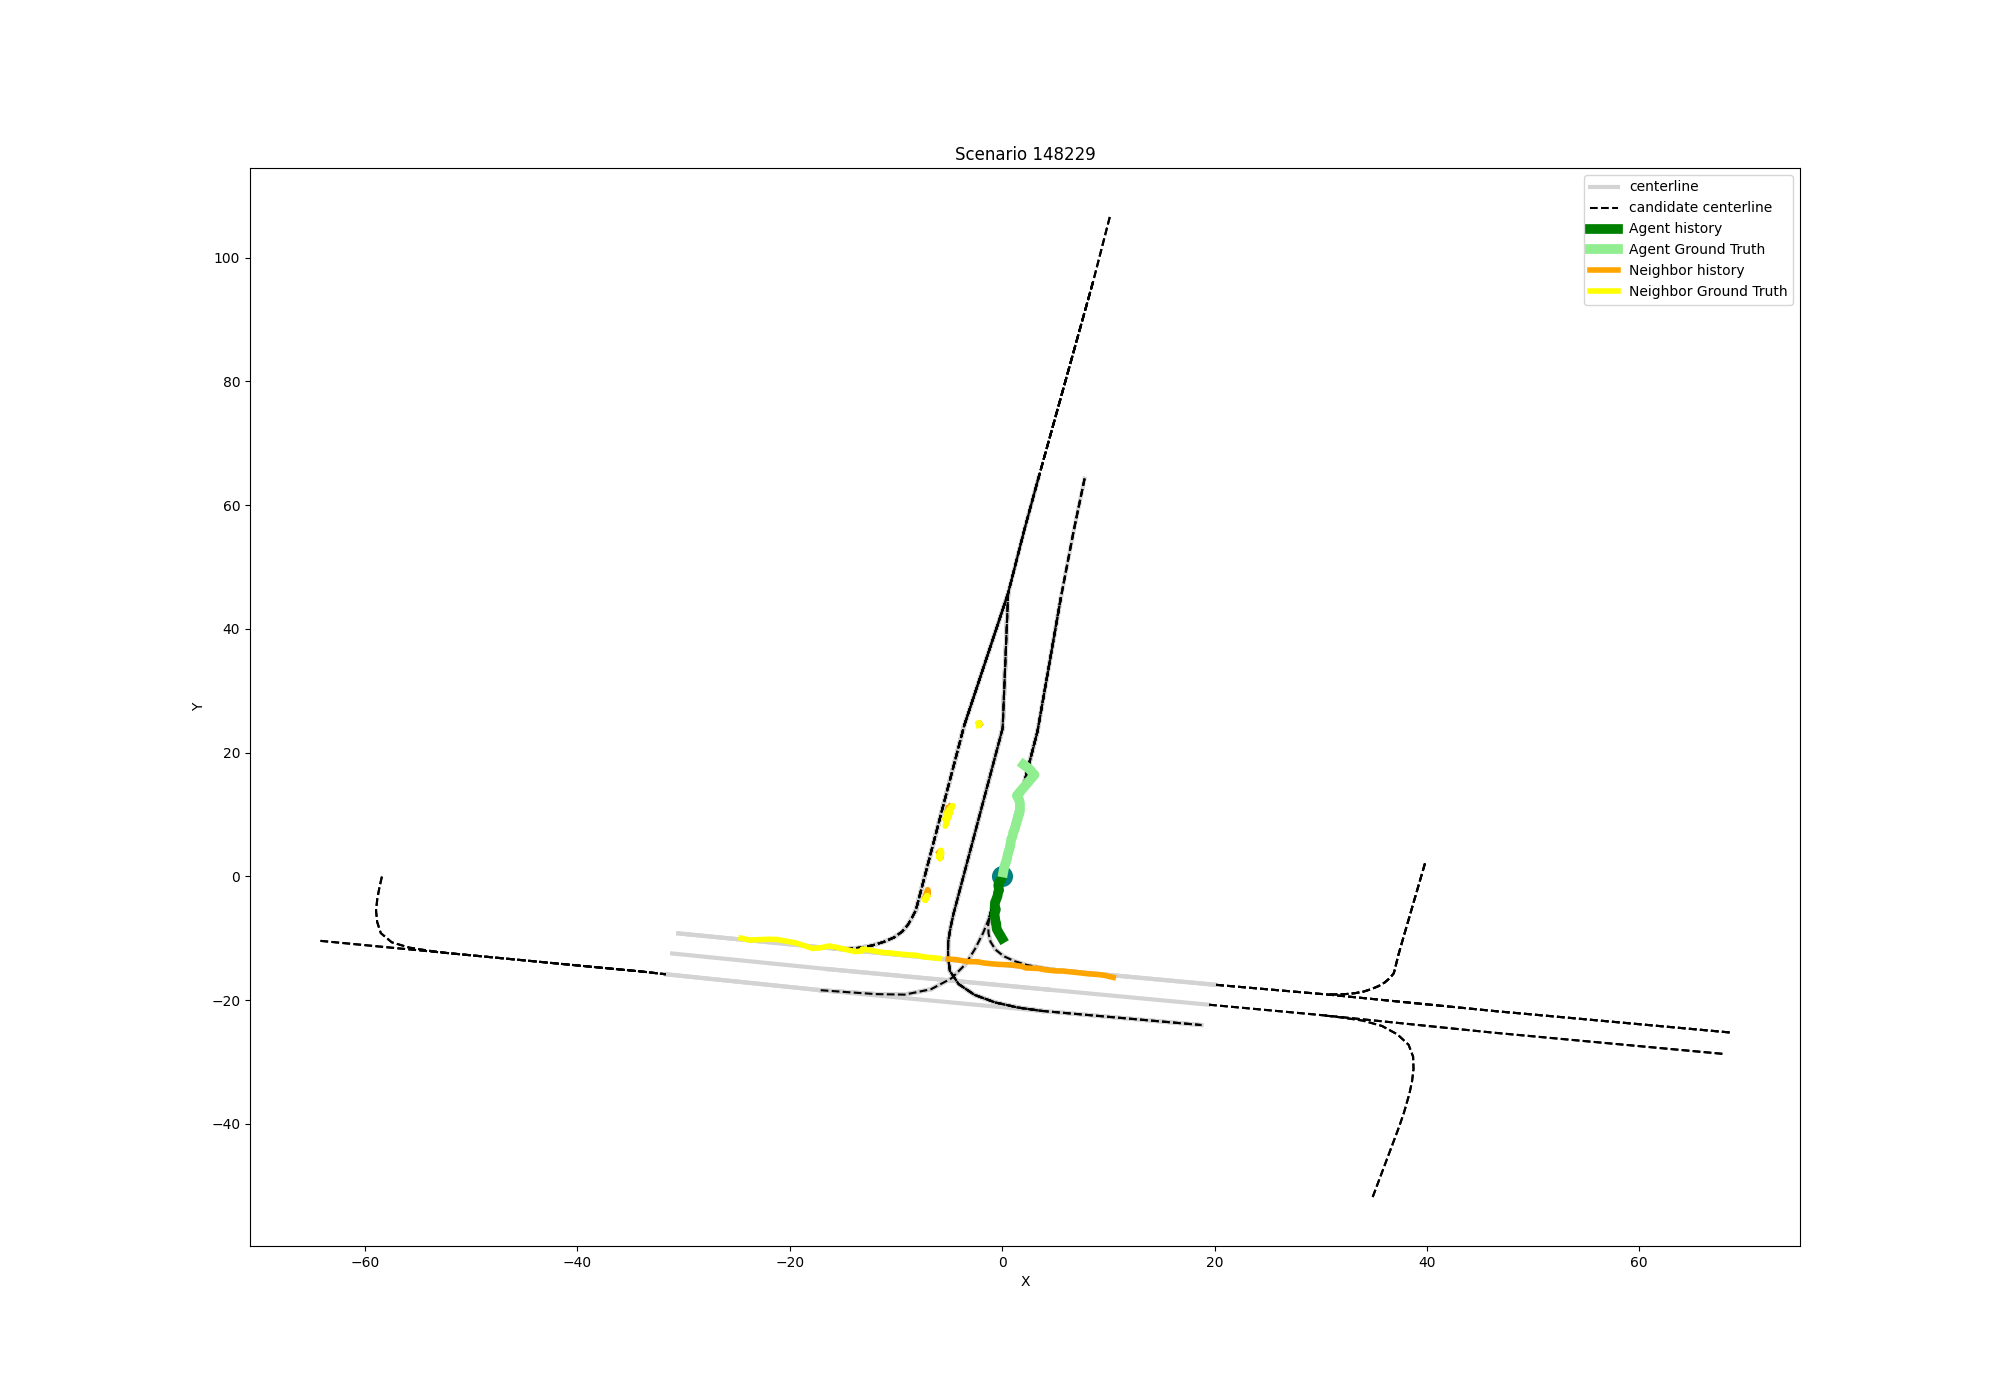
\includegraphics[width=0.9\textwidth]{images/scenario_148229.png}
  \caption{Визуализација припремљених података - Пример 1 (TODO: Ажурирати слике)}
  \label{scenario-example-148229}
\end{figure}

\begin{figure}[H]
  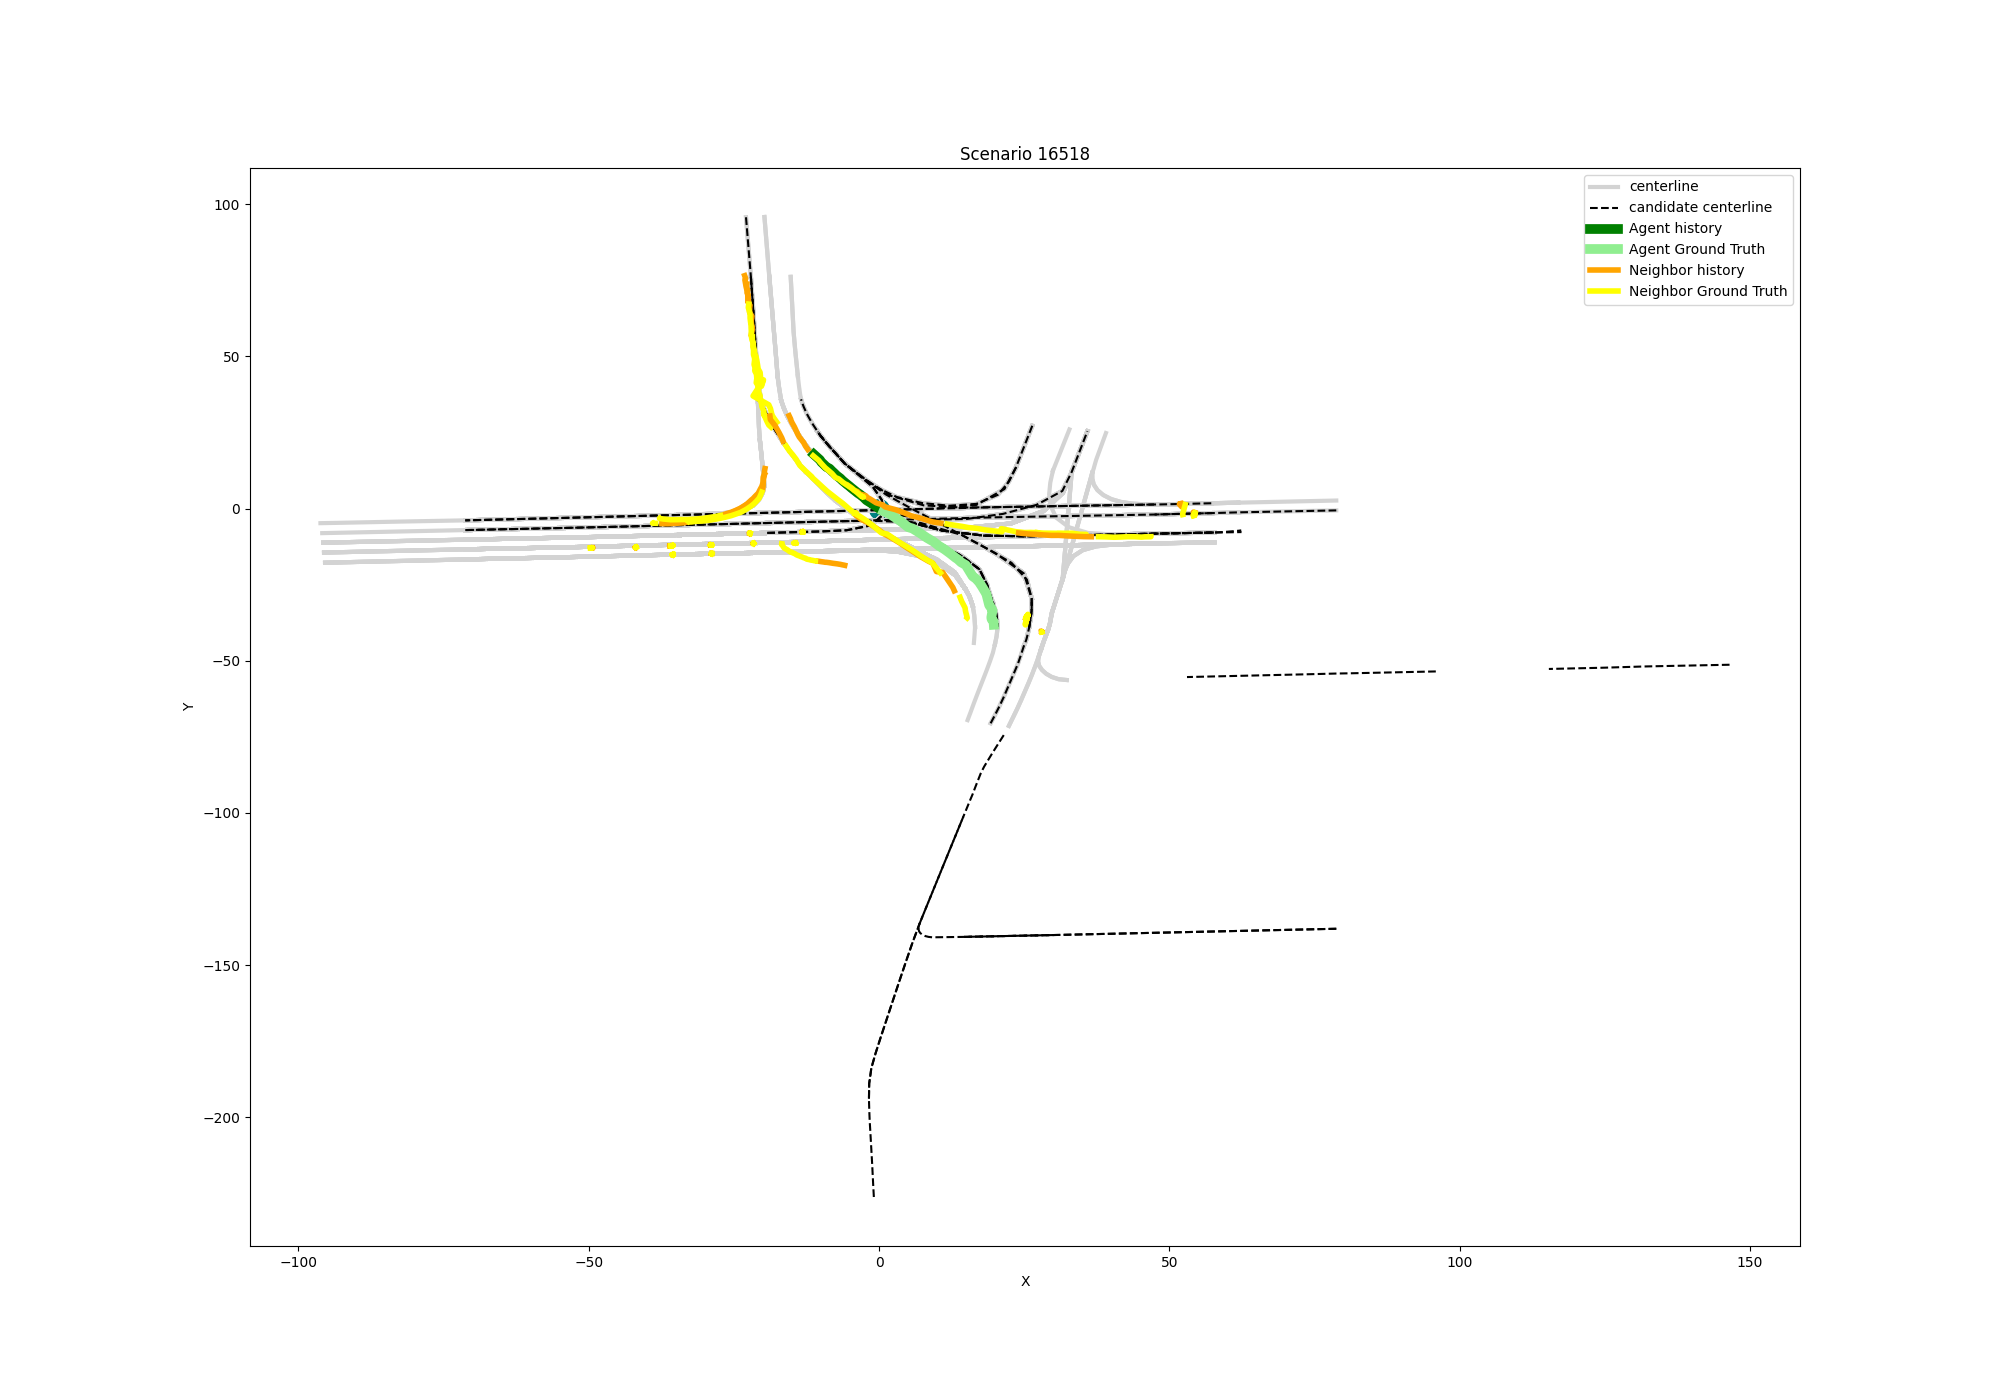
\includegraphics[width=0.9\textwidth]{images/scenario_16518.png}
  \caption{Визуализација припремљених података - Пример 2 (TODO: Ажурирати слике)}
  \label{scenario-example-16518}
\end{figure}

% ------------------------------------------------------------------------------
\chapter{Техника заснована на разумевању контекста обрадом сцене представљене графом}
\label{chp:razrada}
% ------------------------------------------------------------------------------

Независно од конкретног скупа података \textit{HD} мапа, сваки сценарио може да се представи графовском структуром која повезује тачке на сцени, где
свака тачка има своја својства. Свака трајекторија може да се посматра као усмерена сложена незатворена линија (\textit{eng. polyline}) тј. 
низ тачака тако да су сваке две суседне тачке у низу спојене једном усмереном дужи. Тој сложеној линији одговара граф у којем свака тачка
чини чвор, а усмерене дужи чине гране. Како већина елемената \textit{HD} мапа може да се представи сложеном линијом, граф чини идеалну структуру
за представљање једног сценарија. Граф може да се посматра на два нивоа, где се први, нижи ниво односи на топологији сложених линија, а други, виши ниво 
се односи на на везе између сложених линија тј. сложене линије чине чворове у том графу. На овај начин је дефинисана хијерархија графа. 
У наставку се граф на првом нивоу назина подграф, а граф веза између сложених линија се назива глобални граф интеракција (односи се на интеракције
између различитих сложених линија на сцени).

Сценарио из \textit{Argoverse} скупа података се састоји из трајекторија агента, трајекторија суседа, путних сегмената и кандидата путних сегмената.
Како путни сегмент чини специјалну врсту трајекторија, јасно је да сви елементи сценарија могу да се представе сложеним линијама, а самим тим
цео сценарио може да се представи као претходно поменути граф. На слици \ref{polylines-representation} се налази пример једног сценарија
представљен преко сложених линија.

\begin{figure}[H]
  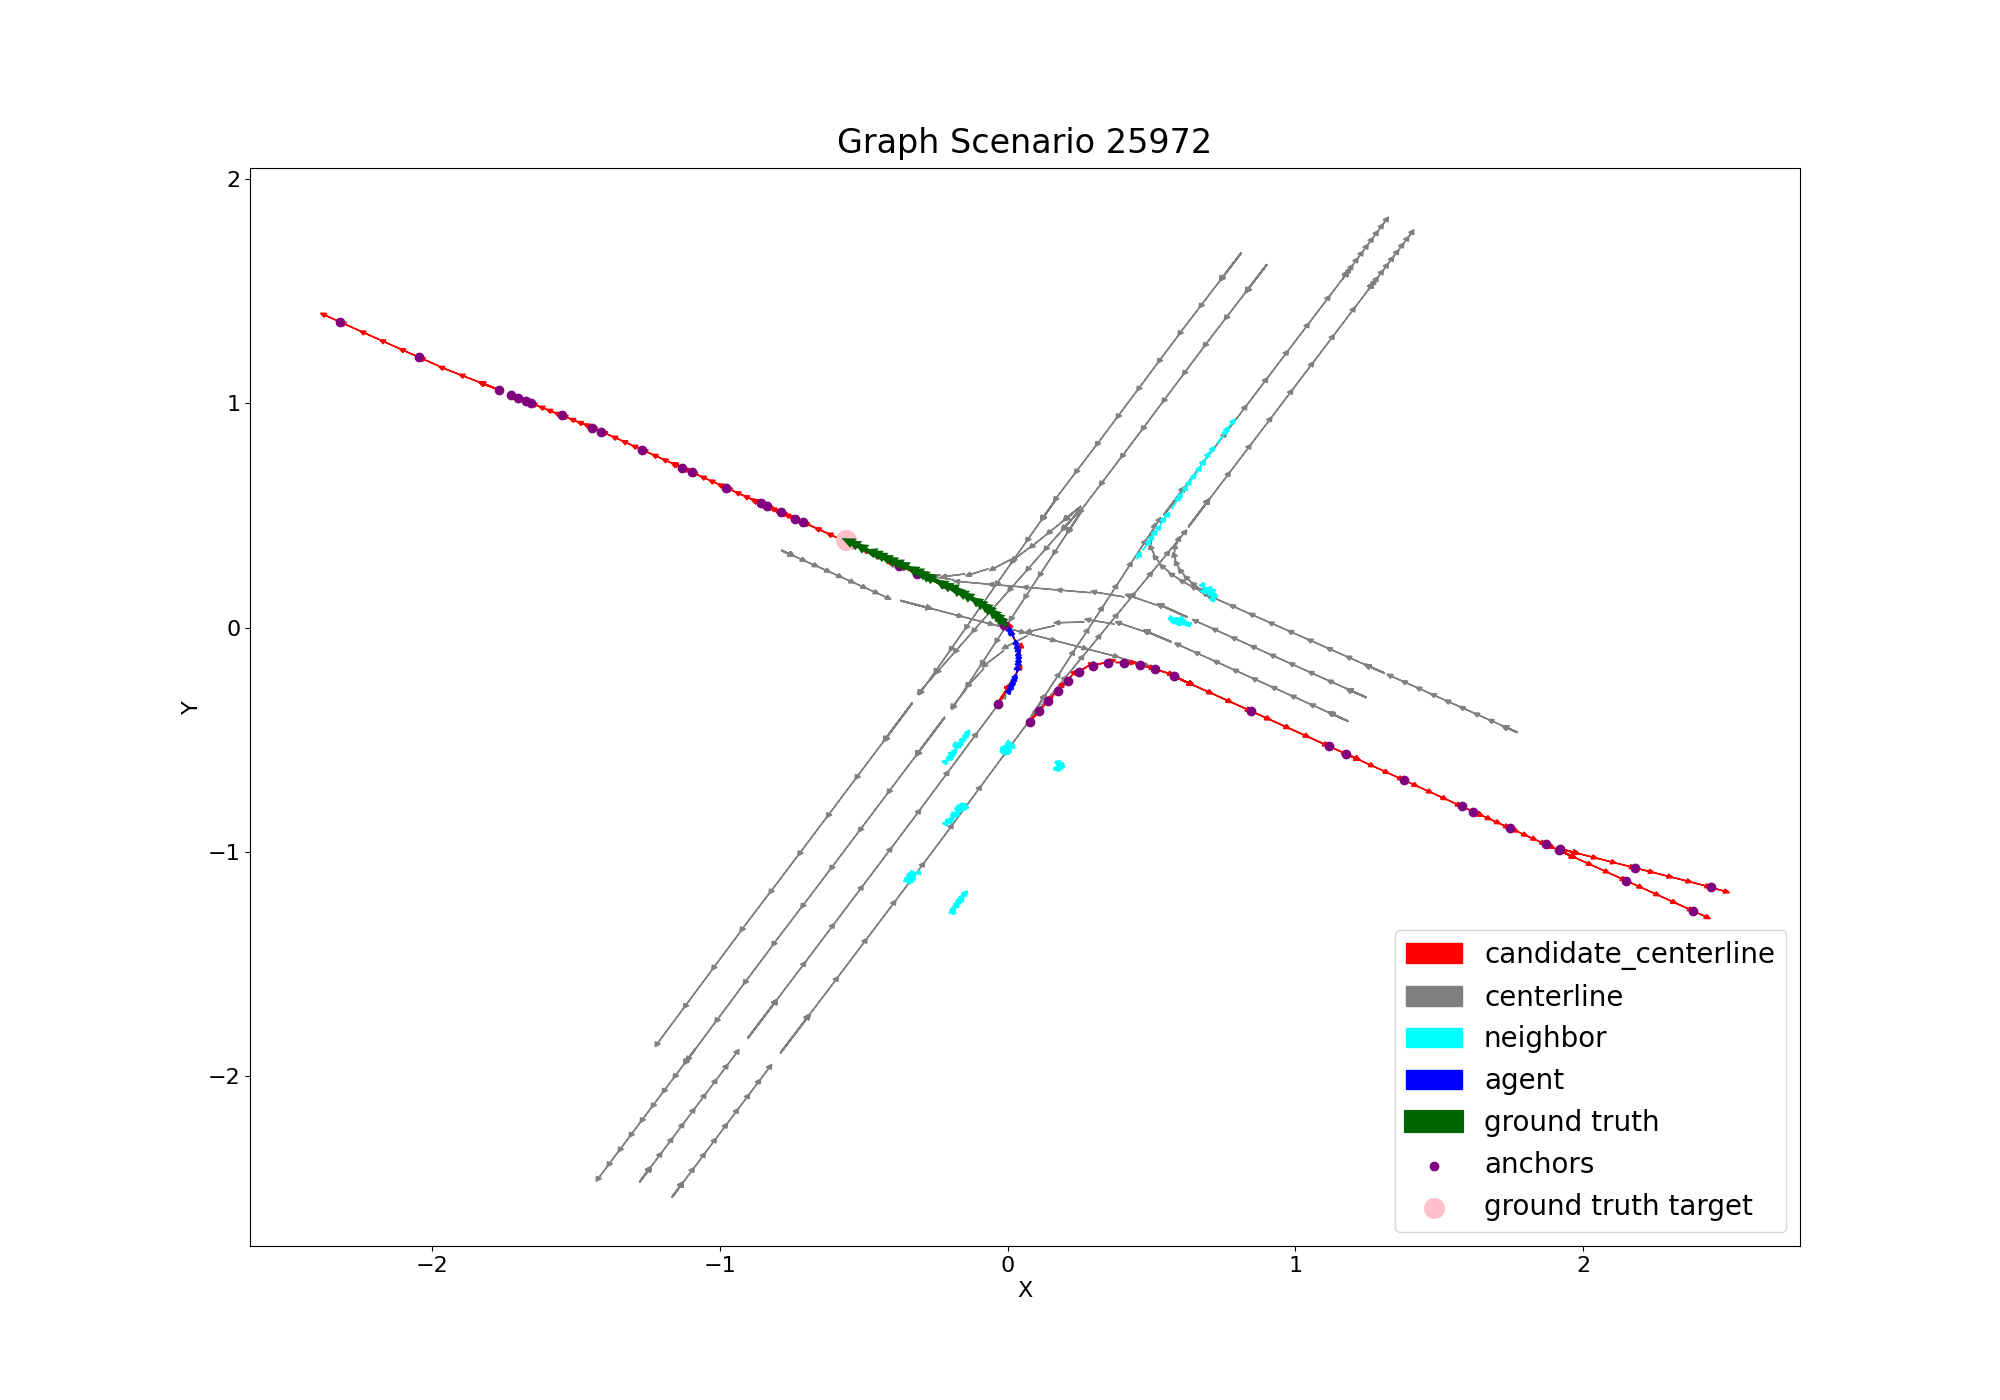
\includegraphics[width=1.0\textwidth]{images/polylines-representation.png}
  \caption{Визуализација репрезентације сложеним линијама}
  \label{polylines-representation}
\end{figure}

\section{Модел \textit{VectorNet}}

\textit{VectorNet} је хијерархијска графовска неуронска мрежа која као улаз добија претходно дефинисани граф на два нивоа, а као резултат
даје предикције трајекторија за све изабране агенте. Архитектура може да генерише предикције за више агената у исто време и то
је погодно искористити у случају да координатни систем сценарија није већ прилагођен конкретном агенту. У супротном је погодније
да се користи итеративни приступ генерисања предикција. 

У наставку ове и осталих секција ће бити описана комплетна архитектура и начин тренирања ове неуронске мреже. Модел се састоји из три компоненте,
чији називи одговарају структури комплетног графа који се користи \cite{vectornet}:
\begin{itemize}
  \item Подграф: Агрегација сложених линија у један вектор који се даље посматра као чвор у глобалном графу;
  \item Глобални граф интеракција: Моделовање интеракција на високом нивоу у глобалном графу помоћу механизма пажње;
  \item Предикција трајекторија за чворове глобалног графа који одговарају агентима.
\end{itemize}

\subsection{Подграф}

Свака сложена линија на сцени се посматра као посебан граф. Применом варијанте графовске неуронске мреже
се издвајају битна својства и везе између чворова. Резултат се на крају агрегира како би се добио један вектор који представља репрезентацију
те сложене линије.

Модел подграфа је варијанта \textit{GCN} архитектуре \cite{gcn} са више слојева. Визуализација једног слоја се види на слици \ref{vectornet-subgraph}. 
Сваки слој може да се представи следећом формулом:

\begin{figure}[H]
  \centering
  $v^{(l+1)}_{i} = \rho_{rel}(g_{enc}(v^{(l)}_{i}),\ \rho_{agg}(A, \{g_{enc}(v^{(l)}_{j})\})))$
\end{figure}

Овде је $v^{(l)}_{i}$ вектор својства чвора из претходног слоја ($v^{(0)}_{i}$ су улазна својства), $g_{enc}$ слој за кодирање својства чвора, 
$\rho_{agg}$ операција агрегације порука добијених од суседних чворова, $A$ je матрица повезаности сложене линије, 
а $\rho_{rel}$ операција обједињавања агрегираних порука суседа и својства самог чвора. Избор операција је произвољан.

\noindent Конкретно \cite{vectornet}:
\begin{itemize}
  \item $g_{enc}$ је потпуно повезана неуронска мрежа;
  \item $\rho_{agg}$ је максимум свих порука од суседа (\textit{max pool}) (TODO: тренутно је avg pool);
  \item $\rho_{rel}$ је конкатенација својста чвора и агрегираних порука;
  \item \textit{A} је у оригиналном раду матрица повезаности потпуно повезаног графа. Алтернативе су повезаност једног чвора са следећим 
  или свим следећим у сложеној линији. 
\end{itemize}

\noindent Вектор сложене линије се добија агрегацијом добијеног графа последњег слоја. За агрегацију се опет користи \textit{max pool} 
функција:

\begin{figure}[H]
  \centering
  $P_{feat} = \rho_{agg}(\{v^{(L)}_{i}\})$
\end{figure}

На слици \ref{vectornet-subgraph} је визуализован цео процен трансформације који се примеђује над подграфом. Процес на слици се односи на само
једну итерацију трансформације, али може бити више идентичних итерација.

\begin{figure}[H]
  \centering
  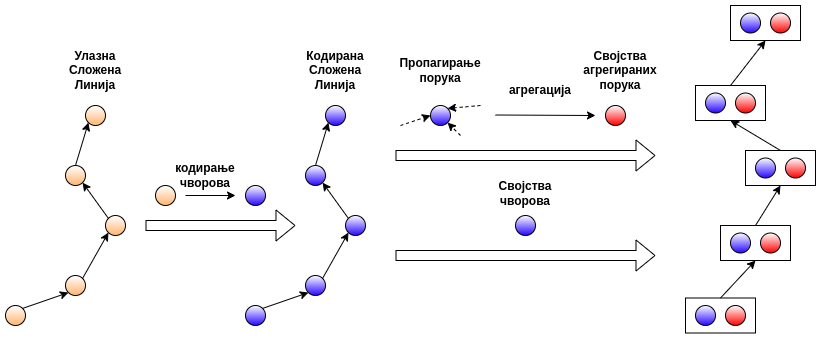
\includegraphics[width=0.9\textwidth]{images/vectornet-subgraph-rs.drawio.png}
  \caption{Визуализација једног слоја \label{vectornet-subgraph}}
\end{figure}

Из угла имплементације, улаз у ову компоненту модела је вектор димензије $(B, P, T, F)$, где је $B$ димензија подскупа података једног корака, 
$P$ је број сложених линија у једном графу, $T$ је дужина сложене линије, a $F$ је број својстава. Након $L$ слојева се добија вектор димензије 
$(B, P, T, F \cdot 2^{L})$ који се агрегира на нивоу чворова на вектор димензије
$(B, P, F \cdot 2^{L})$\footnote{Претпоставка је да свака сложена линија има исти број својстава и да сваки граф има исти број сложених линија}. 
Агрегирану сложену линију посматрамо као један чвор у глобалном графу.
         
\subsection{Глобални граф интеракција}

Глобални граф интеракција се посматра као класичан граф са матрицом повезаности \textit{A} преко које може да се дефинише хеуристика, као што је на пример удаљеност
чворова на сцени. У оригиналном раду се ради једноставности глобални граф посматра као потпуно повезан граф без тежина \cite{vectornet}.

Циљ глобалног графа интеракција је разумевање интеракција између агената и осталих објеката на сцени. Механизмом пажње се примењује над 
чворовима глобалног графа и проналазе везе између чворова графа \cite{attention_is_all_you_need}. Интуиција је да се на овај начин проналазе путни сегменти који најбоље одговарају будућој трајекотрији агента и 
одређивање суседних објеката који утичу на само кретање агента. Не постоји ограничење на избор неуронске мреже која се примењује на глобални граф.

\begin{figure}[H]
  \centering
  $\{P^{(l+1)}_{i}\} = GNN(\{P^{(l)}_{i}\}, A)$
\end{figure}

\noindent Конкретно у имплементацији се користи следећи облик. Скалирање је опционо.

\begin{figure}[H]
  \centering
  $GNN = softmax(\frac{P_{Q}P^{T}_{K}}{\sqrt{d_{K}}})P_{V}$
\end{figure}

Овај и претходни слој модела чине енкодер, чији је циљ разумевања контекста сцене на висиком нивоу. Последњи слој је декодер
који се односи на предикцију трајекторија.

\subsection{Предикција трајекторија}

За предикцију трајекторија се филтрирају чворови агената из глобалног графа интеракције. За сваког агента се примењује призвољан декодер модел
чији је излаз предикција трајекторије. Наједноставнији приступ је коришћење потпуно повезане неуронске мреже под претпоставком да су 
тачке трајекторије међусобно независне. Овај корак се замењује напреднијим приступоп у модификованој верзији заснованој на узоркованим циљним тачкама.

\subsection{Функција грешке}

За функцију грешке предикције трајекторија $L_{traj}$ се користи \textit{huber} функција грешке тј. комбинација \textit{L1} и \textit{L2} функције грешке 
(TODO: opisati huber funkciju greske negde.). 
У процесу тренирања може да се дода задатак \textbf{естимације недостајућих чворова глобалног графа интеракција}. Насумично се бирају чворови у графу и замаскирају
се његова својства (множењем са нулом). Сваком чвору се додају две ,,нове`` вредности које су једнаке минималној вредности свакој од координата почетних 
тачака сложене линије\footnote{Опис својстава сложених линија је описан у секцији за припрему података}. Нове вредности представљају идентификаторе
тих сложених линија који се користе приликом тренирања модела за естимацију недостајућих својстава чворова. Циљ овог задатка је форсирање бољег разумевања
веза између трајекторија и генерално веза између сложених линија у графу. Функција грешке овог задатка ($L_{node}$) се имплементира коришћењем \textit{L1}
функције грешке \cite{vectornet}.

\begin{figure}[H]
  \centering
  $L = L_{traj} + \alpha \cdot L_{node}$
\end{figure}

\section{Модификована верзија \textit{VectorNet} са узоркованим крајњим тачкама трајекторија}

Претходно поменута верзија \textit{VectorNet} модела може да се унапреди додавањем доменског знања. Један приступ је да се користе унапред
дефинисани предлози трајекторија који се користе као основе за генерисање предикција трајекторија. Предлози су фиксни током процеса
предвиђања и биарају се на основу анализе података и кластеровањем свих трајекторија \cite{multipath}.
Ова метода је аналогна примени предлога (,,сидра`` - \textit{eng. anchors}) која се користи код детекције објеката.

Алтернатива која се исто заснива на предлозима (,,сидрима``) је да се уместо предлога трајекторија користе предлози крајњих тачака трајекторија
тј. циљних тачаја. Модел који генерише трајекторију на основу циљне тачке и својства из \textit{VectorNet} се тренира слично као и основни модел, 
али квалитет целог система доста зависи од квалитета узорковања тих предлога. Алгоритам за узорковање предлога је већ објашњен у секцији за
иницијалну припрему података.

Архитектура \textit{TNT: Target-driveN Trajectory prediction} \cite{tnt} се заснива баш на тој идеји и подразумева следеће кораке:
\begin{enumerate}
  \item Разумевање контекста помоћу \textit{VectorNet} модела (основа архитектуре);
  \item Генерисање корекција \textit(eng. offsets) и поузданости за сваки предлог циљне тачке трајекторије;
  \item Узорковање модификованих предлога на основу поузданости;
  \item Естимација трајекторије до сваког изабраног предлога крајње тачке.
  \item Естимација вероватноће за сваку од добијену трајектору (TODO: Trenutno se koriste verovatnoce krajnih tacaka);
  \item Филтрирање трајекторија на основу вероватноћа (TODO).
\end{enumerate}

На слици \ref{tnt-viz-1} су представљени кораци 2 и 3 под претпоставком да је корак 1 претходно извршен. На сцени се налазе два агента 
\textit{1} и \textit{2}. Мали љубичасти кругови се односе на предлоге циљних тачака који су узорковани са кандидата путних сегмената
у процесу припреме података (TODO: Opis pripreme je na kraju, ali verovatno treba ranije...). Сви се налазе на централним линијама, 
јер се узоркују са центра путних сегмената. Сви кругови су означени тако да је јасно ком агенту припадају. На основу поузданости је 
извршено филтрирање иницијалних предлога, због чега су неки кругови избељени. За остале кругове постоје корекције\footnote{
  У имплементацији се у једном кораку генеришу корекција и поузданост за све узорковане циљне тачке, али овде су због прегледности
  избачене корекције за одбачене предлоге.
} (наранџасти кругови спојени са иницијалним предлогом).


\begin{figure}[H]
  \centering
  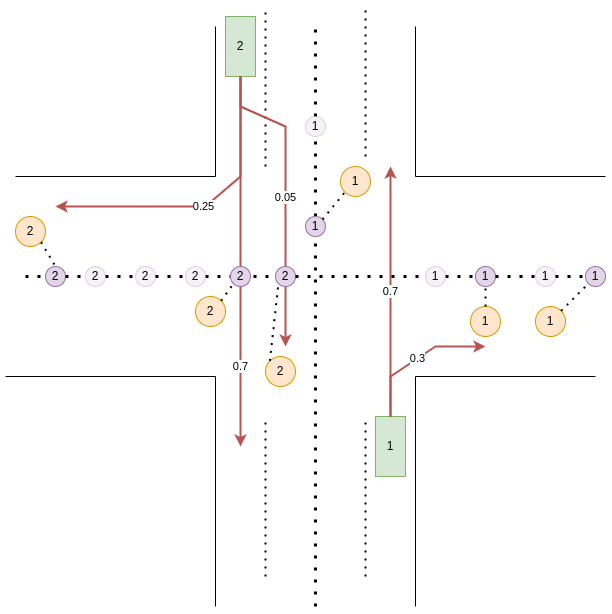
\includegraphics[width=0.6\textwidth]{images/tnt-viz-Page-1.drawio.png}
  \caption{Визуалиција \textit{TNT} - фаза 1 \label{tnt-viz-1}}
\end{figure}

На основу ових коначних циљних тачака се врши предвиђање трајекторија и то је приказано на слици \ref{tnt-viz-2}. Крај предвиђене трајекторије не мора
нужно да се поклапа са циљном тачком.

\begin{figure}[H]
  \centering
  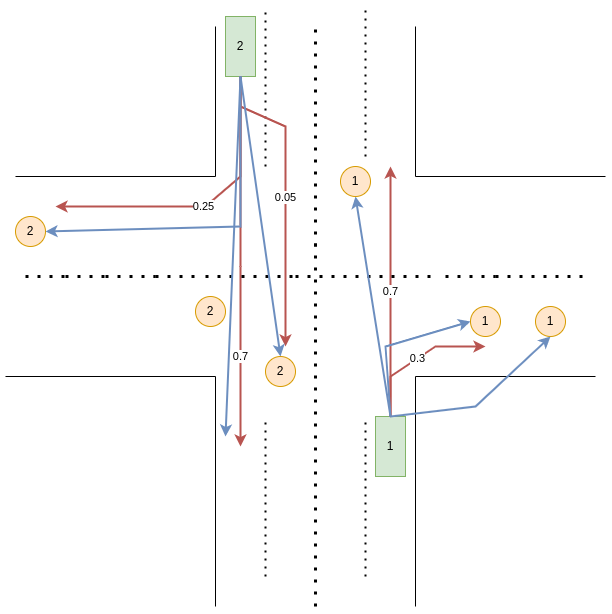
\includegraphics[width=0.6\textwidth]{images/tnt-viz-Page-2.drawio.png}
  \caption{Визуалиција \textit{TNT} - фаза 2 \label{tnt-viz-2}}
\end{figure}


Уместо последња два корака могу да се користе вероватноће (поузданости) предлога крајњих тачака, али из добре крајње тачке не следи
нужно квалитетна трајекторија (нпр. уколико предложена трајектрорија прелази преко тротоара). На слици \ref{tnt-good-target-bad-traj}
је дат такав пример. Овде је зелени правоугаоник агент, црвена трајекторија је истинита вредност трајекторије која се предвиђа, 
наранџасти круг је циљна тачка, а плава трајекторија је предикција. 

\begin{figure}[H]
  \centering
  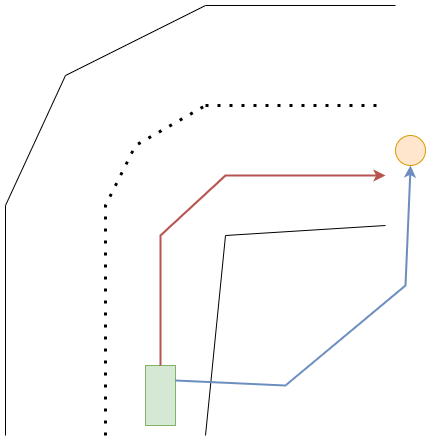
\includegraphics[width=0.5\textwidth]{images/tnt-good-end-point-and-bad-traj.drawio.png}
  \caption{Пример случаја где је добра циљна тачка, а лоша трајекторија \label{tnt-good-target-bad-traj}}
\end{figure}

Овде \textit{VectorNet} чини језгро архитектуре, а сви наредни кораци могу да се имплементирају потпуно повезаним неуронским мрежама уз комбинацију
једноставних детерминистичких алгоритама. Главни изазов ове архитектуре је у алгоритму за генерисање предлога
\footnote{Алгоритам је укратко описан у секцији за иницијалну припрему података} и балансирању
параметара функција грешака приликом учења модела.

\noindent Ако се не учи \textit{естимације недостајућих чворова глобалног графа интеракција} уз \textit{VectorNet}, 
онда функција грешке има следећи облик:

\begin{figure}[H]
  \centering
  $L = \lambda_{1} \cdot L_{offsets} + \lambda_{2} \cdot L_{tarconf} + \lambda_{3} \cdot L_{trajde} + \lambda_{4} \cdot L_{trajconf}$
\end{figure}

Нека је $P_{anchors}$ скуп свих предлога крајњих тачака трајекторија и нека је $P_{gt}$ истинита крајња тачка трајекторије. Тада се изваја
из скупа $P_{anchors}$ елемент $P_{closest}$ који је најближи истинитој крајњој тачки\footnote{Овде не узимамо у обзир поправке, 
већ нетрансформисане, узорковане вредности. 
Уколико се у обзир узимају вредности са поправкама, онда процес учења постаје тежак због шума (мења се индекс најближе тачке). Ово можда не би био
толики проблем да су остале трајекторије другачије дефинисане тј. независне од промене изабране, најближе тачке.}. 
Тада је:

\begin{figure}[H]
  \centering
  $L_{offsets} = H_{delta}(P_{closest\_offset}, \hat{P}_{closest\_offset})$
\end{figure}

\noindent где је $H_{delta}$ \textit{huber} функција грешке са параметром \textit{delta}, $P_{closest\_offset} := P_{gt} - P_{closest}$,
а $\hat{P}_{closest\_offset}$ је предикција тог одступања. Циљ је да баш тај најближи предлог има највећу поузданост, па се функција грешке за 
поузданост дефинише на следећи начих:

\begin{figure}[H]
  \centering
  $L_{tarconf} = BCE(P_{closest\_onehot}, \hat{P}_{confs})$
\end{figure}

\noindent где \textit{BCE} је бинарна унакрсна ентропија, $P_{closest\_onehot}$ индекс елемента $P_{closest}$ у \textit{onehot} 
формату\footnote{Индекс се представља као низ димензије броја класа (предложених крајњих тачака у овом случају) где су свуда нуле сем на локацији која одговара
вредности тог индекса.} и $\hat{P}_{confs}$ поузданост модела за сваки предлог (за сваки предлог се даје поузданост из интервала $[0, 1]$). Функција грешке за
трајекторије је аналогна као и за предлога крајњих тачака. Састоји се из функције грешке за одступање трајекторија од реализације и оцене
поузданости модела за сваку од тих трајекторија.

\begin{figure}[H]
  \centering
  $L_{trajde} = H_{delta} (T_{traj}, \hat{T}_{traj})$
\end{figure}

\noindent где је $T_{traj}$ истинита вредност трајекторије, а $\hat{T}_{traj}$ је њена предикција. Приликом учења се за естимацију трајекторије 
$\hat{T}_{traj}$ узима истинита крајња тачка трајекторије како би учење било стабилније. Ова техника се зове ,,Учитељско форсирање`` \cite{teacher_forcing}.
Последња компонента се односи на поузданост модела за сваку естимацију трајекторија. За сваку естимирану трајекторију се рачуна максимално растојање 
између свих упарених тачака естимиране трајекторије и истините вредности трајекторије тј. 
$D(T_{traj}, \hat{T}_{raj}) := max(||T^{k}_{traj} - \hat{T}^{k}_{traj}||^{2}_{2})$. Тада се ,,истинита расподела`` $P_{traj\_confs}$ одређује као \textit{softmax} 
ових негативних вредности.

\begin{figure}[H]
  \centering
  $L_{trajconf} = BCE(P_{traj\_confs}, \hat{P}_{traj\_confs})$
\end{figure}

\section{Припрема података}

Припрема података у овој секцији се наставља на иницијални процес претпроцесирања података и своди се на трансформацију свих елемената
\textit{HD} мапа у сложене линије. Да би било могуће спојити више сценарија у један подскуп података за једну итерацију тренирања, неопходно
је да се испуне одређена ограничења:
\begin{itemize}
  \item Сваки сценарио мора да има исти број сложених линија ($N_{p}$). Ако је број сложених линија већи од $N_{p}$, онда се 
        вишак сложених линија одбацује, при чему се води рачуна о приоритету сложеих линија: агент, остали објекти, путеви, путеви кандидати.
        Ако је број сложених линија мањи од $N_{p}$, онда се скуп допуњава сложеним линијама са нула чворовима.
  \item Свака сложена линија мора да има исти број чворова ($N_{n}$). Ово се решава аналогно броју сложених линија.
  \item Сваки чвор сложених линија мора да има исти број својстава ($N_{f}$). Сваки чвор има иста својства, са тим
        да се својства допуњавају нулама ако немају смисла за тај тим сложених линија (агент и путеви немају иста својства).
\end{itemize}

\noindent Сваки чвор сложене линије има следећа својства:
\begin{itemize}
  \item Координате \textit{x} и \textit{y}: Просек претходне и тренутне тачке трајекторије - 2 скалара;
  \item Смер по \textit{x} и \textit{y}: Разлика тренутне и претходне тачке трајекторије - 2 скалара;
  \item Тип објекта као \textit{onehot} вектор (агент, сусед - објекат, пут, пут кандидат) - 4 скалара;
  \item Метаподаци путних чворова (нуле у случају трајекторија агента и објеката суседа)
    \begin{itemize}
      \item Да ли се сегмент пресеца са неким другим сегментом - 1 скалар;
      \item Да ли постоји контрола саобраћаја - 1 скалар;
      \item Смер као \textit{onehot} вектор (нема, десно, лево) - 3 скалара
    \end{itemize}
  \item Да ли је чвор прави (1) или вештачки (0) - 1 скалар.
\end{itemize}

Коначан формат улазних података у \textit{VectorNet} је $(B, N_{p}, N_{n}, 14)$, где је $B$ број сценарија у једном подскупу података,
а $N_{p}$ и $N_{n}$ су параметри.

\section{Експерименти и резултати}

На слици \ref{tnt-scenario-171255} је приказан пример примене \textit{TNT-VectorNet} архитектуре. 

\begin{figure}[H]
  \centering
  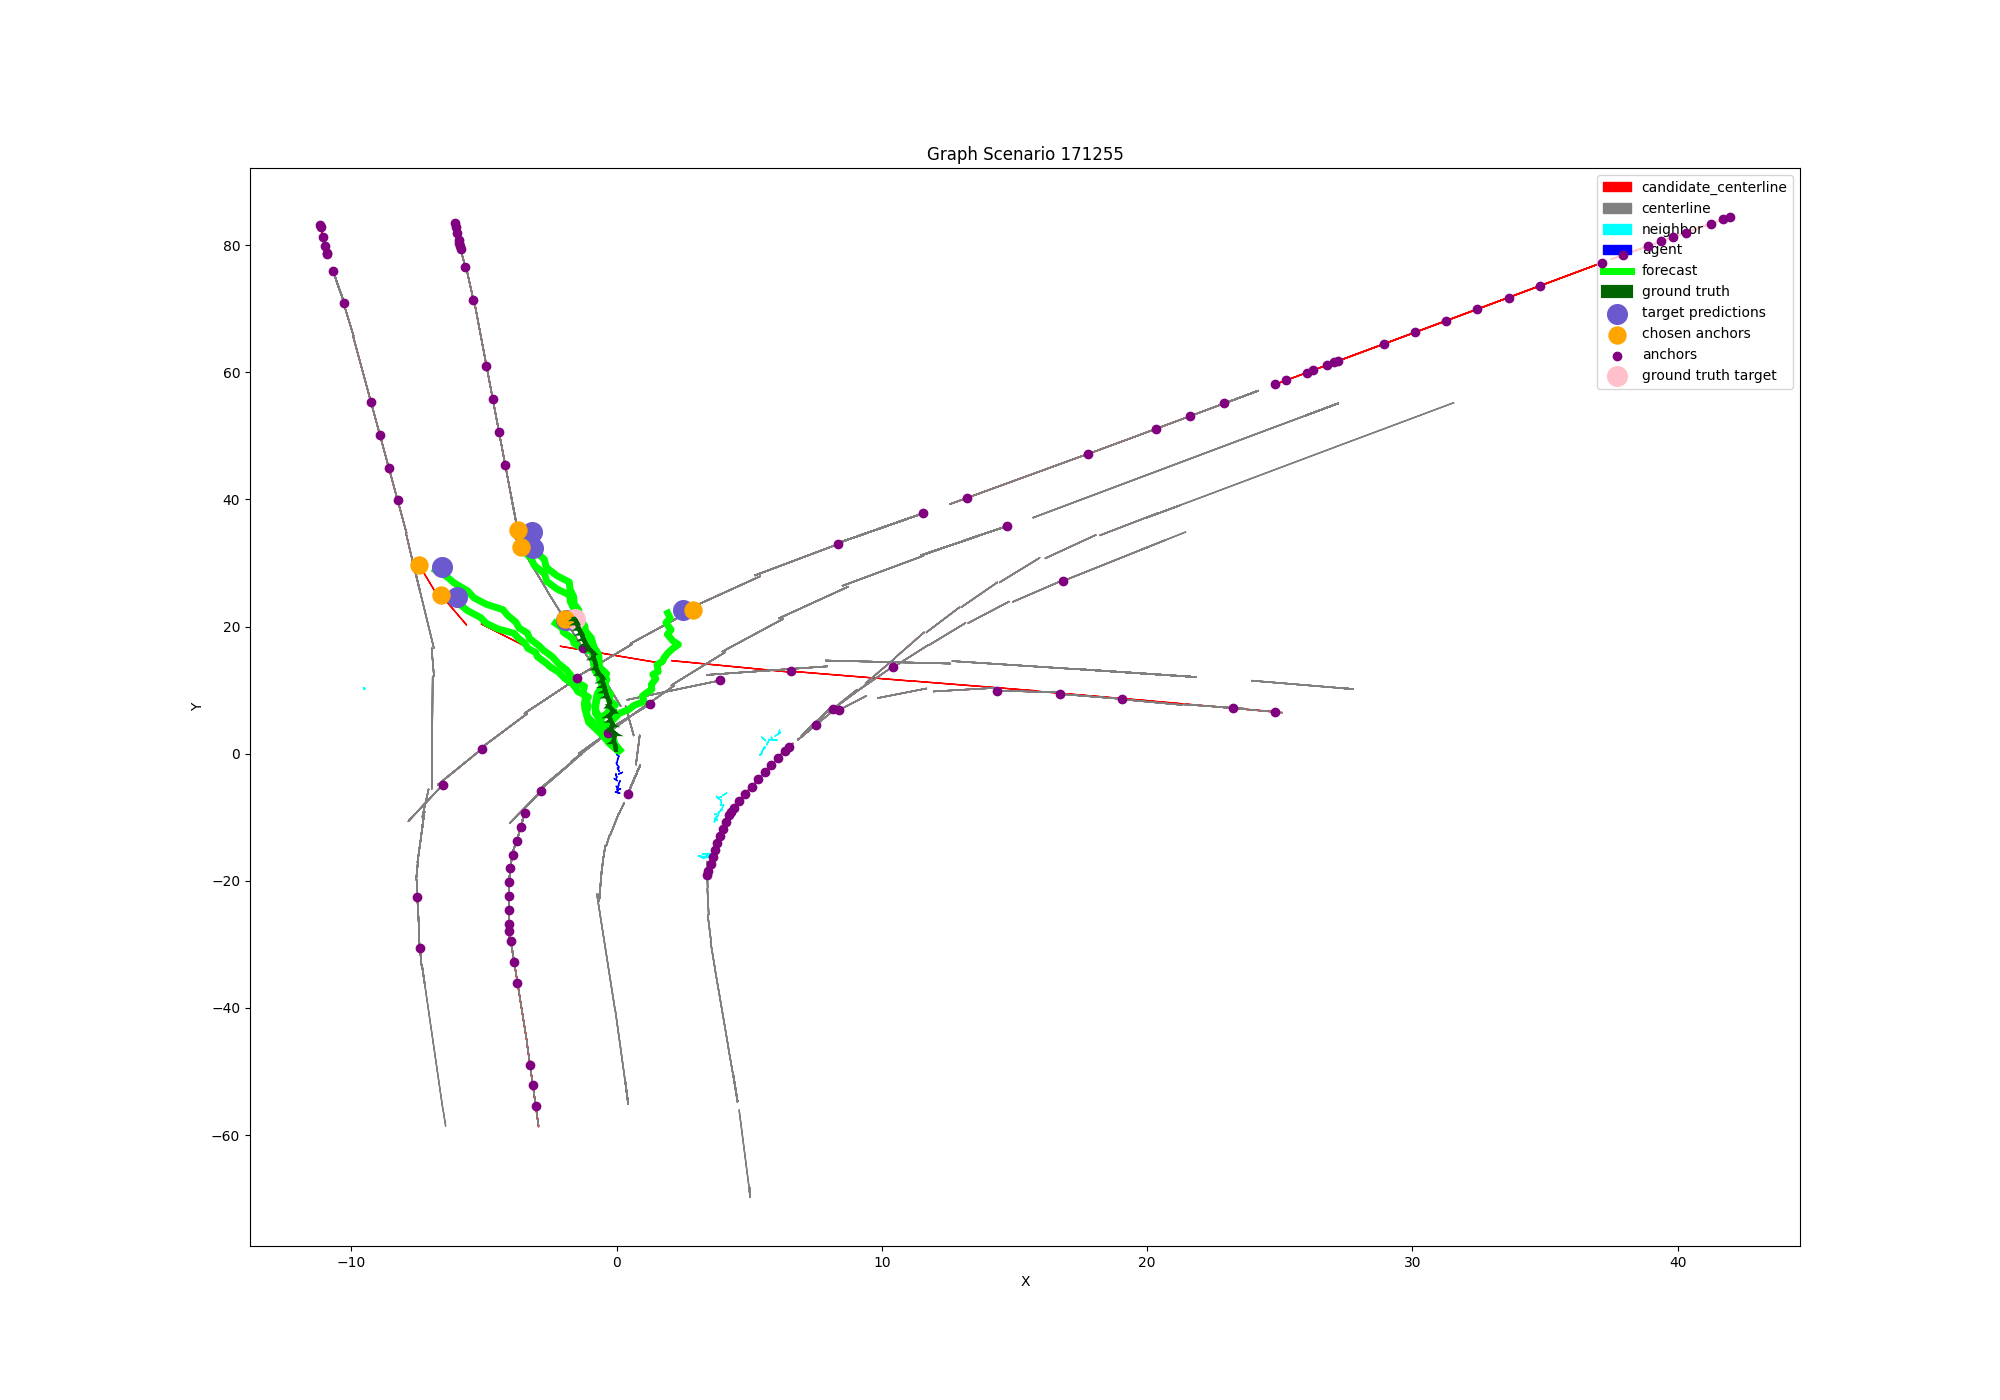
\includegraphics[width=0.9\textwidth]{images/tnt-scenario-171255.png}
  \caption{
    Пример резултата за сценарио 171255 - $minADE_{6} = 0.6, minFDE_{6} = 1.0$. Сивом 
    бојом су обојени путеви, тамно плавом је обојена историја трајекторија агента, светло плавом су обојене историје суседних објеката,
    црвеном линијом су обојени путеви кандидати. Мали љубичасти кругови су узорковани предлози, велики плави кругови су изабрани
    узорковани предлози са највећом поузданошћу, а велики наранџасти кругови су модификовани изабрани предлози. Светло зеленом
    бојом су представљене предикције за сваку од изабраних крајњих тачака, а тамно зеленом бојом су обојени истинити резултати. 
    \label{tnt-scenario-171255}
  }
\end{figure}

У табели \tref{vectornet-results} се налазе резултати репродукованих и модификованих верзија (TODO) \textit{TNT-VectorNet} модела. TODO: Тренутни модел је трениран укупно 1h над свим подацима...

\begin{table}
  \begin{tabular}{c|c|c}
    Назив модела & \textit{minADE} (6) & \textit{minFDE} (6) \\
    \hline
    \textit{TNT-original без оцене трајекторија} & 0.877 & 1.632 \\
    \textit{TNT-original са оценом трајекторија} & 0.728 & 1.292 \\
    \textit{TNT-custom без оцене трајекторија}  & 1.19 & 2.25
  \end{tabular}
  \caption{Резултати}
  \label{vectornet-results}
\end{table}

У наставку су изабране слике које укратко описују неке од врлине и мана основног модела. На слици \ref{tnt-MIA-34142} модел даје
6 трајекторије за 6 изабраних по моделу најпоузданих тачака од 50 генерисаних (исти параметри су и за остале слике). Три трајекторије
се завршавају у околини истините крајње тачке, што даје добре резултате на овом конкретном сценарију. Поред тога постоје
2 трајекторије које одговарају случају скретања и то представља добар одговор на изазов мултимодалности. Последња трајекторије
нема смислену крајњу тачку и скреће са пута. Трајекторије су углавном исправне под условом да је крајња тачка добро изабрана.  

\begin{figure}[H]
  \centering
  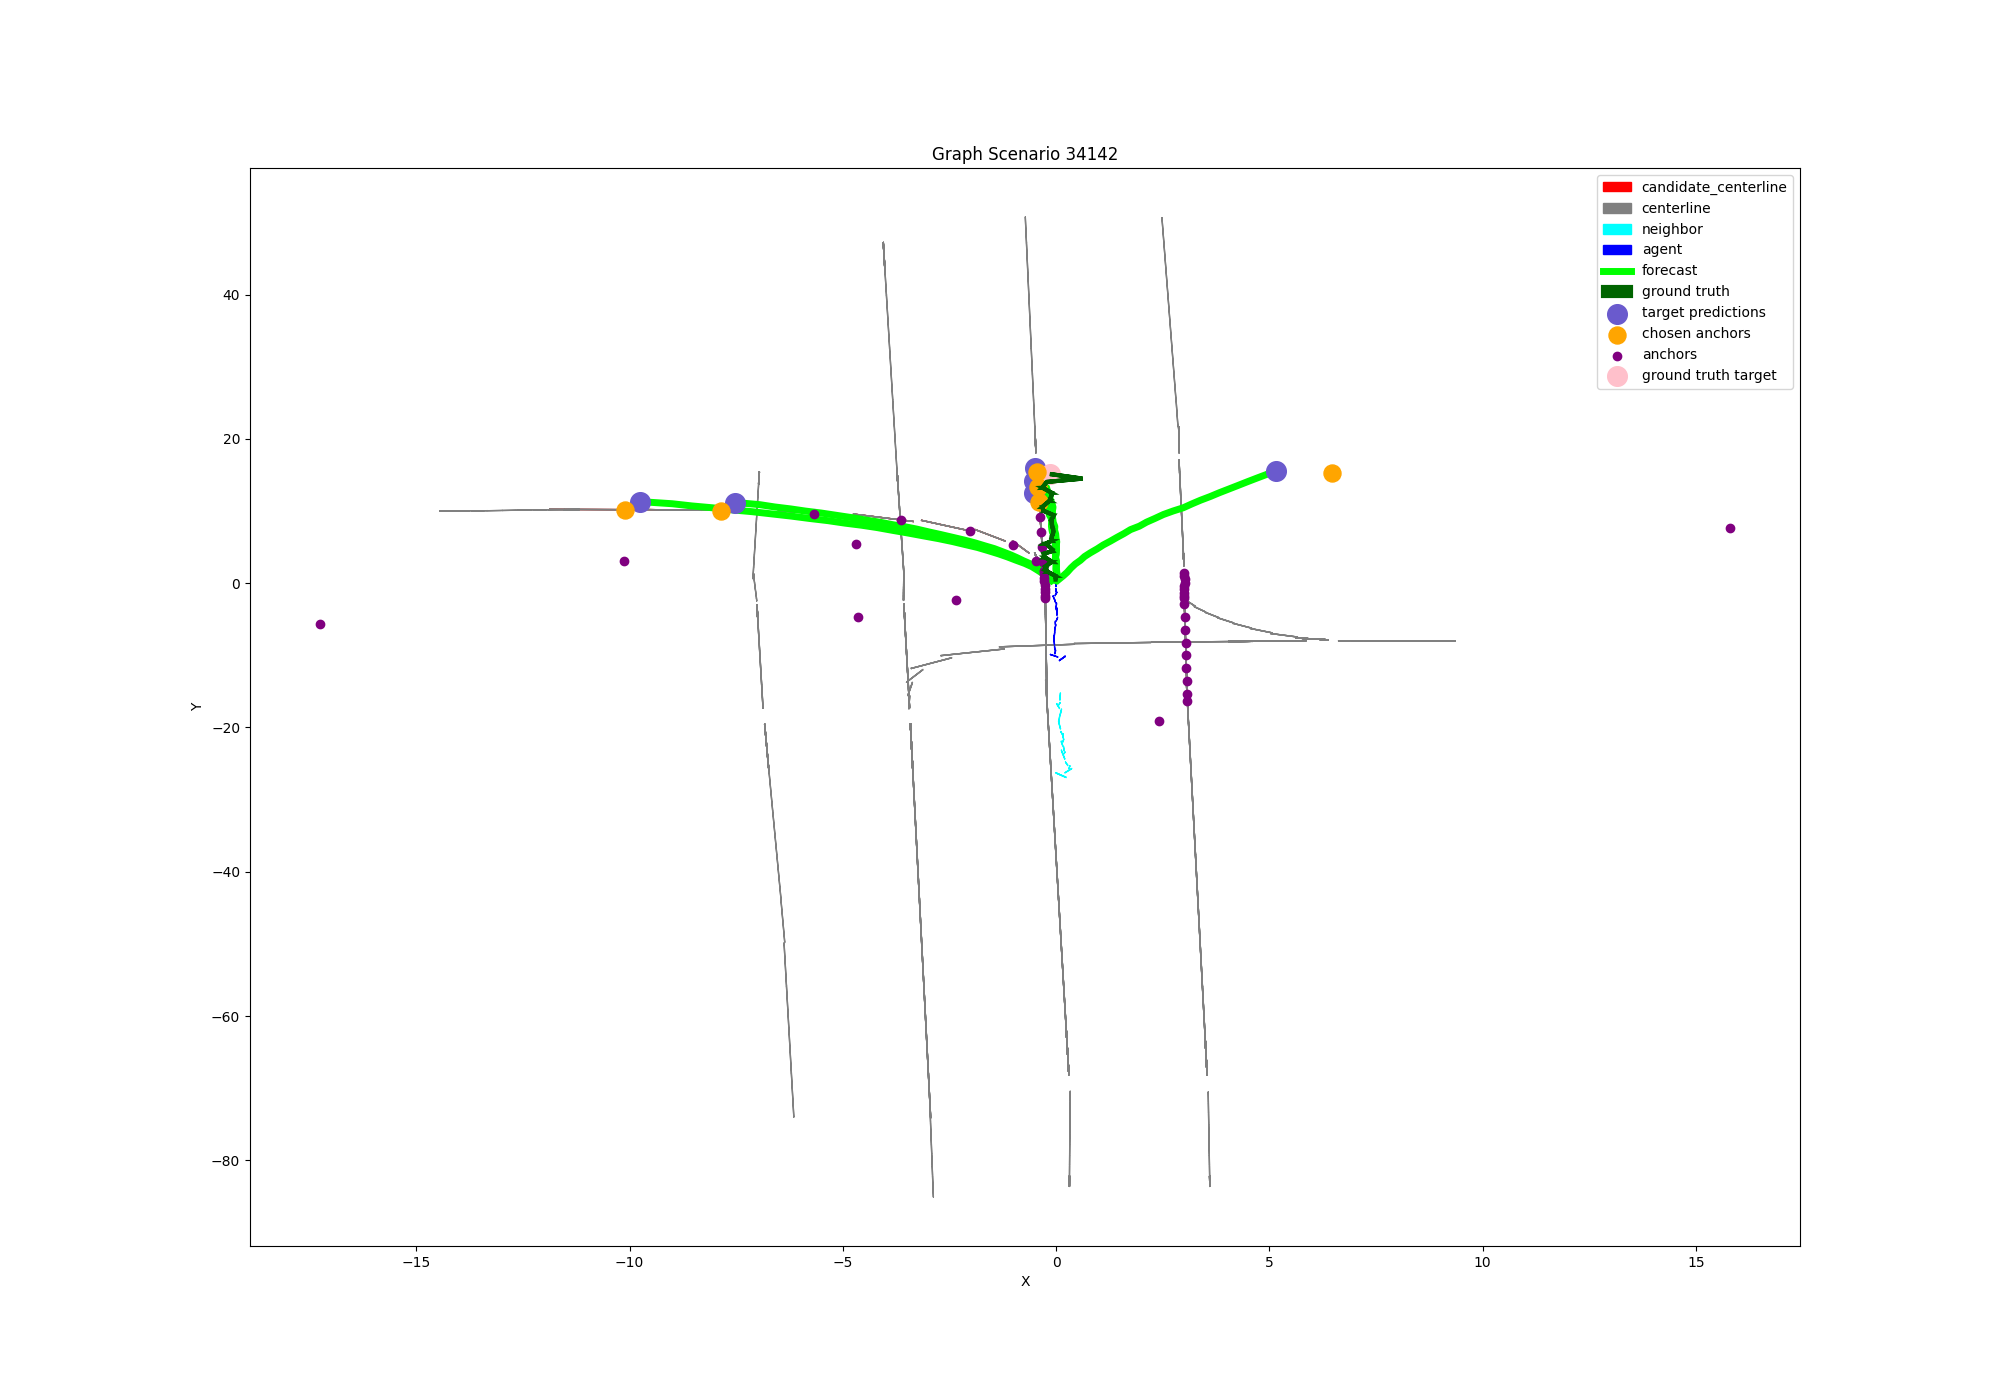
\includegraphics[width=1.0\textwidth]{images/MIA_34142.png}
  \caption{Предикције на сценарију \textit{MIA-34142} \label{tnt-MIA-34142}}
\end{figure}

Сценарио на слици \ref{tnt-MIA-92250} приказује случај где су предлози крајњих тачака јако лоши (део сценарија је лоше исечен), али 
модел и даље успева да модификује те крајње тачке (претпостака је да је то на основу трајекторије историје) и да добар резултат.

\begin{figure}[H]
  \centering
  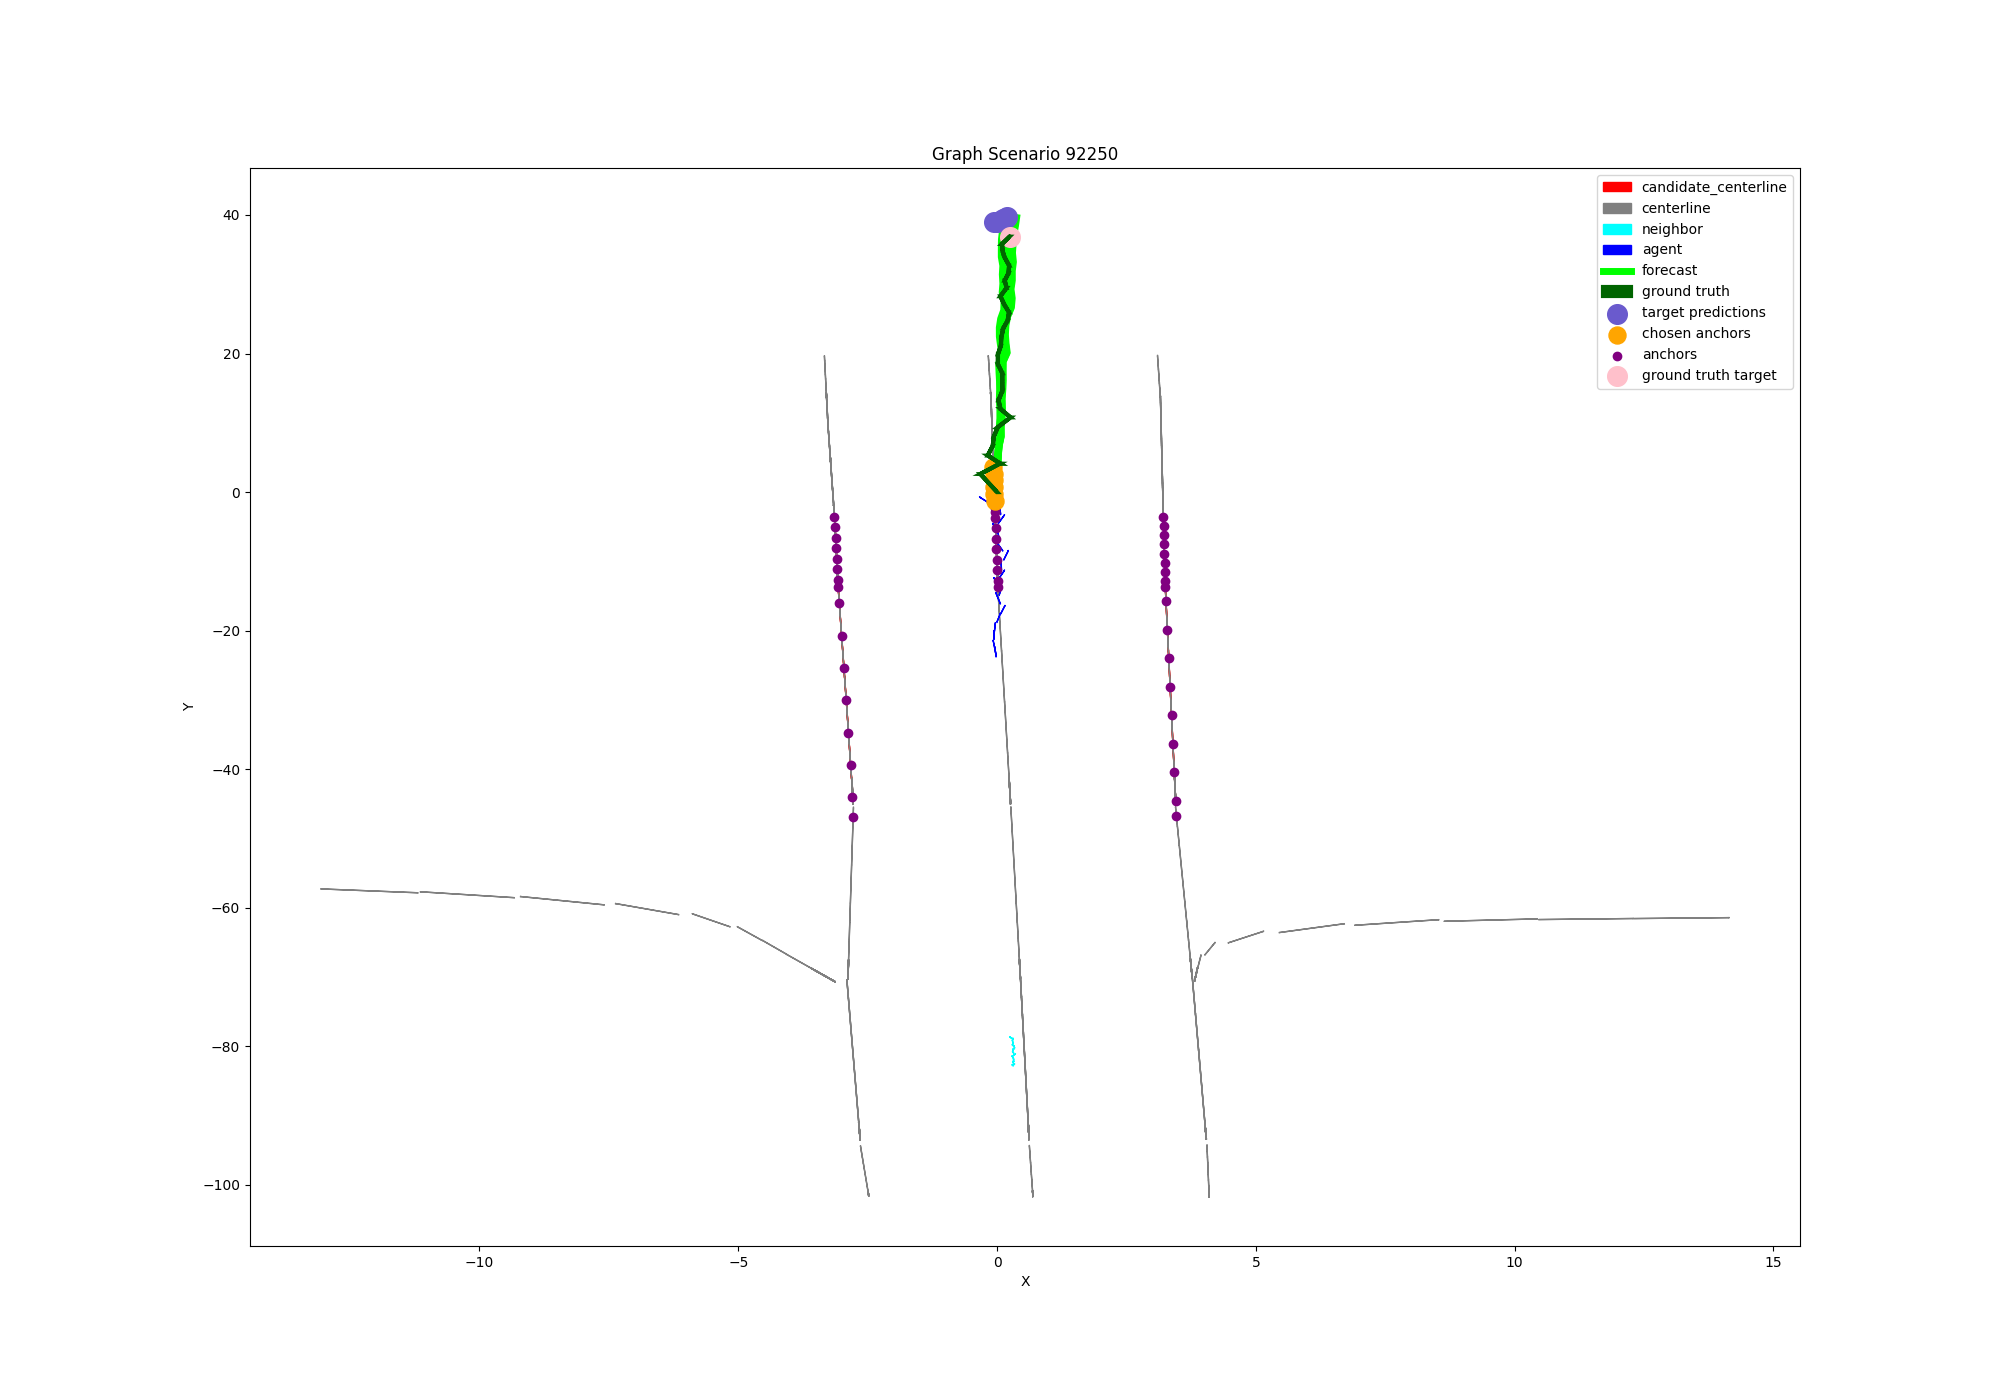
\includegraphics[width=1.0\textwidth]{images/MIA_92250.png}
  \caption{Предикције на сценарију \textit{MIA-92250} \label{tnt-MIA-92250}}
\end{figure}

Сценарио на слици \ref{tnt-MIA-189984} приказује јако лоше одговоре који су последица лошег алгоритма узорковања предлога (кандидата). Мана
наивног приступа, где се за путни сегмент агента одређује онај који је најближи последњој тачки трајекторије. У случаје грешке се добијају
кандити на путевима који су усмерени на супротну страну. Квалитет модела значајно зависи од алгоритма узорковања иницијалних предлога 
крајњих тачака.

\begin{figure}[H]
  \centering
  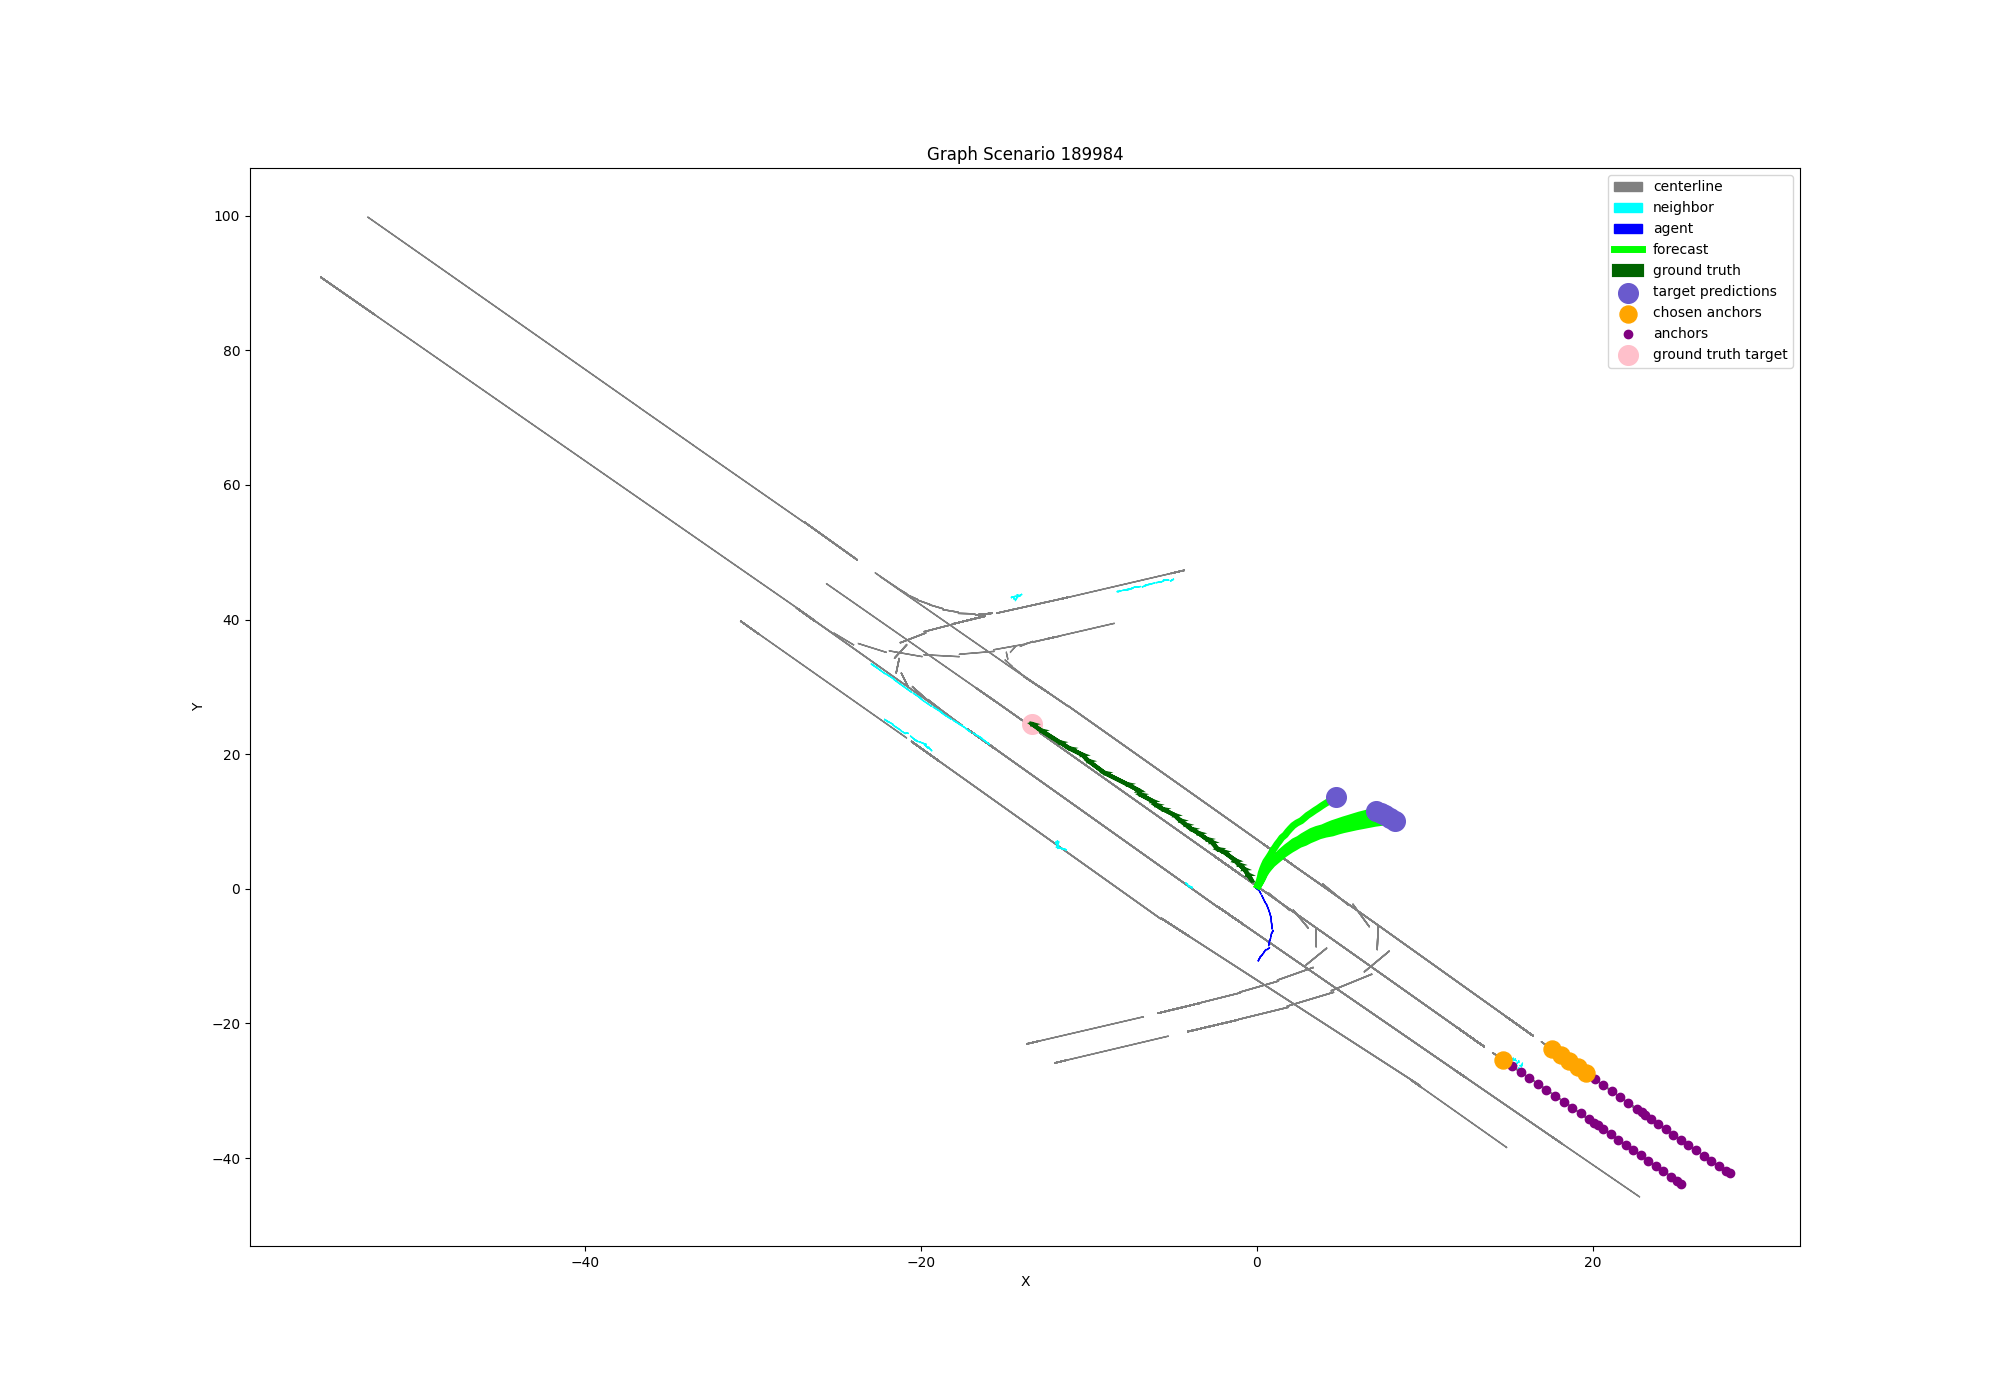
\includegraphics[width=1.0\textwidth]{images/MIA_189984.png}
  \caption{Предикције на сценарију \textit{MIA-189984} \label{tnt-MIA-189984}}
\end{figure}

% ------------------------------------------------------------------------------
\chapter{Техника заснована на разумевању контекста обрадом растеризоване сцене}
\label{chp:razrada}
% ------------------------------------------------------------------------------

Алтернативни приступ структуирања података \textit{HD} мапа је њихова растеризација. Како су коришћени подаци
сцене из птичје перспективе тј. дводимензионалном облику, онда је природно да се мапе посматрају као слике. Стандардне слике
се представљају као матрица пиксела, где сваки пиксел има једну вредност (један канал) у случају црно белих слика или 
три вредности (три канала) у случају да су слике у \textit{RGB} формату којим се представља боја пиксела. У случају \textit{HD}
мапа, не користе се боје, већ се сваком пикселу додељују својства сцене као што су: да ли се на датој позицији налази агент,
да ли постоји контрола саобраћаја, да ли је могућа вожња на тој локацији и слично. Процес трансформације \textit{HD} мапе у 
слику се у наставку реферише као растеризација \textit{HD} мапе. 

Када су подаци у облику слика, тада је могућа примена конволутивних неуронских мрежа са циљем извлачења контекста из растера. У овој секцији се
примеђује \textit{HOME} \cite{home} архитектура која имплементира предикцију трајекторија кроз у три фазе: генерисање топлотне мапе 
вероватноћа крајњих тачака тачака трајекторије, узорковање крајњих тачака на основу топлотних мапа и естимација трајекторије до задате крајње
тачке. 

У наставку се описује припрема података. Након примпреме података је детаљно описана архитектура.

\section{Растеризација \textit{HD} мапа}

Овај корак припреме података се наставља на иницијалну припрему и секцији \ref{initprep} исто као и припрема података за \textit{Vectornet} модел. 
Овај корак припреме захтева онлајн приступ припреме због димензије података након конверзије.
\footnote{онлајн припрема подрзумева да се подаци припремају упоредо са тренирањем модела.} 
Растеризован облик чини
низ ретких матрица (већина вредности је нула), због чега он може да буде и до 200 пута веће димензије од основног облика. За чување
целог свих слика је потребно око \textit{4TB}. Овакав начин припреме не утиче значајно на дужину трајања једне епохе током тренирања. Иницијална
припрема се и даље врши офлајн. Исти приступ је могуће искористити и за \textit{VectorNet}, али у том случају није од толиког значаја. 

У \textit{Argoverse} скупу података су познате комплетне сцене градова, а за генерисање предикција конкретног агента у конкретном тренутку је
потребан само један исечак града у облику квадрата центриран у односу на агента. 
Димензија тог квадрата је значајан параметар за припрему података и сам модел. Квадрат треба да буде довољно велики да обухвати скоро сваку
трајекторију у скупу података. Дужина већина трајекторија је краћа од 56 метара што чини 112 пиксела у \textit{Argoverse} скупу података. Због
тога се за исечак узима квадрат димензије $(224, 224)$ центриран у односу на последњу познату локацију агента. Овај исечак са издвојеним
одговарајућим својствима у сваком пикселу чини улаз у модел за генерисање топлотне мапе вероватноћа крајњих тачака. У имплементацији
страница квадрата представља параметар који је подесив.

Коначан облик једне слике је $(10, 224, 224)$, где је $10$ низ својстава пиксела. Сваки пиксел садржи следеће информације:
\begin{itemize}
  \item Да ли локација пиксела припада путу тј. да ли је могућа вожња на тој локацији. Информација се бележи бинарно, где
        1 означава да је на тој локацији могућа вожња, а 0 да није могућа вожња.
  \item Растеризована трајекторија агента: Трајекторија агента се растеризује тако што се посматра локација агента
        у сваком тренутку који је забележен у историји трајекторије агента. Тој локацији тј. тим координатама се додељује
        правоугаоник димензије $(S_x, S_y)$. Сваки пиксел који припада том квадрату добија вредност 1 за својство растеризоване
        трајекторије агента. У оригиналној имплементацији се за сваки временски тренутак чува засебна трајекторија. Ради
        уштеде меморије се користи само једно заједничко својство за све тренутке.
  \item Растеризоване трајекторије суседа: Аналогно агенту се растеризују трајекторија осталих објеката на сцени.
  \item Метаподаци путних сегмената: За сваки путни сегмент је дато 5 бинарних својстава:
        \begin{itemize}
          \item да ли путни сегмент припада пресеку путних сегмената;
          \item да ли путни сегмент обухвата контролу саобраћаја;
          \item да ли путни сегмент подразумева скретање у десно;
          \item да ли путни сегмент подразумева скретање у лево;
          \item да ли путни сегмент не подразумева скретање;
        \end{itemize}
        Путни сегменти се посматрају као специјална врста трајекторија, па се растеризују аналогно трајекторији агента.
  \item Растеризовани кандидата путних сегмената: Кандидати путних сегмената на основу којих се узоркују предлози крајњих тачака
        за \textit{VectorNet} се у овом случају користе као својства. 
\end{itemize}

Поред припреме улазних података, се припрема и истините вредности топлотних мапа вероватноћа крајњих тачака. Истинита крајња тачка трајекотрије агента
припада тачно једном пикселу, али непосредно суседни пиксели такође чине добре предикције. У том случају да се користи само један пиксел за истиниту
вредност, модел се подједнако кажњава ако изабаре најгори могући пиксел као и када изабере непосредно суседни пиксел. Из тог разлога се примеђује
гаувом кернел након постављене истините крајње тачке топлотне мапе. Облик топлотне мапе је $(1, 224, 224)$ тј. аналогно улазним подацима. Опционо,
топлотна мапа која се добија као излаз модела може да буде мање димензије, а да се накнадно скалира на одговарајућу димензију.

Архитектура \textit{HOME} поред слике користи и историју агента и осталих објеката у облику временских серија. Ове две структуре података
се комбинују.

% ------------------------------------------------------------------------------
\chapter{Закључак}
% ------------------------------------------------------------------------------
У изради...

% ==============================================================================
% Završni deo teze i prilozi
\backmatter
% ==============================================================================

% Datoteka sa literaturom u BibTex tj. BibLaTeX/Biber formatu
\bibliography{matfmaster-primer}
\bibliographystyle{ieeetr}

% ------------------------------------------------------------------------------
% Biografija kandidata
\begin{biografija}
\textbf{Момир Аџемовић} 
У изради...
\end{biografija}
% ------------------------------------------------------------------------------

\end{document} 